\documentclass[final,5p,times,twocolumn]{elsarticle}
\usepackage[T1]{fontenc}
\usepackage{amsmath,amssymb}
\usepackage{graphicx}
\usepackage[table]{xcolor}
\usepackage{booktabs,tabularx,array}
\usepackage{subcaption}
\usepackage[hyphens]{url}
\usepackage{xurl}
\usepackage{enumitem}
\usepackage{microtype}
\usepackage{fancyhdr}
\usepackage{placeins}
\definecolor{elsevierblue}{RGB}{0,115,152}
\definecolor{proposedrow}{RGB}{226,237,247}
\usepackage[colorlinks=true,linkcolor=elsevierblue,citecolor=elsevierblue,urlcolor=elsevierblue,breaklinks=true]{hyperref}
\urlstyle{same}
\graphicspath{{figures/}}
\raggedbottom
\setlength{\parskip}{0pt}
\setlength{\textfloatsep}{5pt plus 1pt minus 2pt}
\setlength{\dbltextfloatsep}{6pt plus 1pt minus 2pt}
\setlength{\floatsep}{5pt plus 1pt minus 2pt}
\setlength{\intextsep}{5pt plus 1pt minus 2pt}
\setlength{\abovecaptionskip}{3pt}
\setlength{\belowcaptionskip}{2pt}
\setlist{nosep,leftmargin=*}
\setlength{\parindent}{1em}
\emergencystretch=1.5em
\renewcommand{\topfraction}{0.88}
\renewcommand{\bottomfraction}{0.88}
\renewcommand{\textfraction}{0.10}
\renewcommand{\floatpagefraction}{0.86}
\renewcommand{\dbltopfraction}{0.88}
\renewcommand{\dblfloatpagefraction}{0.86}
\newcommand{\proposed}{EF-GBTSVM-PF}
\newcommand{\nz}{\%}
% compact the reference list slightly so it does not spill a near-empty final page
\makeatletter
\let\oldthebibliography\thebibliography
\renewcommand{\thebibliography}[1]{\footnotesize\oldthebibliography{#1}%
  \setlength{\itemsep}{1.4pt}\setlength{\parsep}{0pt}\setlength{\topsep}{2pt}}
\makeatother
\abstracttitle{}
\hypersetup{pdfauthor={},pdftitle={A Leakage-Audited Battery Degradation Classification Benchmark}}
\biboptions{numbers,sort&compress}
\pagestyle{fancy}
\fancyhf{}
\fancyhead[L]{}
\fancyhead[R]{Battery degradation classification under label noise}
\fancyfoot[C]{\thepage}
\renewcommand{\headrulewidth}{0.3pt}
\fancypagestyle{plain}{%
  \fancyhf{}
  \fancyhead[L]{}
  \fancyhead[R]{Battery degradation classification under label noise}
  \fancyfoot[C]{\thepage}
  \renewcommand{\headrulewidth}{0.3pt}}
\begin{document}
\begin{frontmatter}
\title{\textbf{A Leakage-Audited Benchmark of Granular-Ball Twin Support Vector Machines for Battery Degradation Classification under Training-Label Noise}}
\begin{abstract}
\noindent\fbox{\parbox{\dimexpr\textwidth-2\fboxsep-2\fboxrule\relax}{\textbf{HIGHLIGHTS}\par\smallskip
\textbullet\ A record audit removes shared discharge timing and cross-fold variant selection.\par
\textbullet\ Twelve loaded-discharge features are normalised by each cell's label-free first cycle.\par
\textbullet\ Seventeen models are compared at 0\nz, 6\nz\ and an exploratory 6.8\nz\ noise level.\par
\textbullet\ The proposed selector ranks first at both noisy conditions and twelfth on clean labels.}}
\vspace{6pt}\hrule\vspace{7pt}
\noindent\begin{minipage}[t]{.26\textwidth}\raggedright
\textbf{KEYWORDS}\par\smallskip Lithium-ion battery\par State of health\par Granular-ball computing\par Twin support vector machine\par Label noise\par Leave-one-battery-out evaluation\par Data leakage
\end{minipage}\hfill
\begin{minipage}[t]{.70\textwidth}\raggedright
\textbf{ABSTRACT}\par\smallskip
A battery-management system must decide whether a cell is still fit for service or should be retired, and that decision is normally taken at a threshold on state of health (SOH). Close to such a threshold the label itself is uncertain, so a classifier's tolerance to corrupted training labels matters as much as its clean-data accuracy. We study binary degradation classification at SOH $<0.80$ on four NASA PCoE cells under leave-one-battery-out (LOBO) evaluation. An audit of the source records exposed two risks. Cells B0005--B0007 share identical discharge time vectors, so whole-record timing statistics can encode a common recording schedule rather than individual cell behaviour; and choosing a model variant from pooled outer-fold scores would let held-out outcomes influence that choice. We therefore use twelve loaded-discharge physics features --- six measurements and six forms referenced to each cell's own label-free first cycle --- and introduce \proposed, which selects among granular-ball twin-SVM variants using battery-grouped inner validation inside each outer training fold. Seventeen models are compared under a common search budget, with exact-count symmetric label flips applied to training data only. Three conditions are reported: 0\nz\ and 6\nz\ training-label noise, plus a 6.8\nz\ point chosen after the 6\nz\ result had been seen. On clean labels \proposed\ reaches 95.25\nz\ accuracy and ranks twelfth of seventeen: eleven models are ahead of it, led by plain TSVM at 98.77\nz\ and including a single-feature decision stump. At 6\nz\ it reaches 98.01\nz\ accuracy and 98.10\nz\ balanced accuracy, ranking first on both; at 6.8\nz\ it reaches 97.69\nz\ and 97.67\nz, again first. The gap to the best competing model is 3.52 points on clean labels and zero at both noisy conditions. No significance claim accompanies these ranks: four held-out cells put the smallest attainable two-sided $p$-value at 0.125, and the 6.8\nz\ point was not chosen in advance. Every rank reported here is descriptive.
\end{minipage}\par\vspace{7pt}\hrule
\end{abstract}
\end{frontmatter}

\section{Introduction}
Lithium-ion cells power traction, stationary storage and backup systems, and in each of these roles a battery-management system (BMS) has to separate ordinary ageing from a condition that calls for derating, retirement or second-life reuse. Capacity loss is only the most visible symptom of that condition. Interphase growth, lithium plating, loss of active material and rising polarisation all change the voltage and thermal response of a cell before its measured capacity crosses a nominal limit, so a health decision that rests on capacity alone discards information that the discharge curve already contains.

Methods for extracting that information have developed along several lines. Sparse variational Gaussian processes made probabilistic modelling tractable on large records \cite{hensman2015}. Battery diagnostics then used differential thermal voltammetry to resolve health changes directly from measured signatures \cite{merla2016}, examined how temperature gradients drive uneven ageing inside parallel-connected packs \cite{yang2016}, and borrowed scalable tree ensembles such as XGBoost for structured tabular inputs \cite{chen2016xgb}. Taken together these studies argue for physically interpretable signals and for careful treatment of the conditions under which those signals were recorded.

Work published in 2017 and 2018 tied diagnosis more firmly to operational decisions. Degradation diagnostics connected measurable signatures to specific ageing processes \cite{birkl2017}, and battery-reuse research treated cell sorting as an explicit decision problem rather than as a by-product of regression \cite{chen2017reuse}. On the classifier side, twin support vector machines with a pinball loss offered a margin objective that is less sensitive to points near the separating surface \cite{xu2017twin}. Reviews of thermal effects stressed that temperature shapes both ageing and the measured response \cite{ma2018}, while variational Fourier features supplied another route to scalable Gaussian-process inference \cite{hensman2018}.

By 2019 reliability and whole-life reviews had placed ageing mechanisms and safety constraints at the centre of battery assessment \cite{gandoman2019,han2019,li2019}, and early-cycle measurements showed that degradation information is already present long before end of life \cite{severson2019}. In the same year, granular-ball computing proposed replacing pointwise learning with compact groups described by a centre, a radius and a class purity \cite{xia2019gb}. That representation is attractive when labels are imperfect, because a locally consistent group can summarise many observations without treating every individual sample as equally trustworthy.

The 2020 literature broadened the modelling vocabulary further, through reviews of safe battery design \cite{duan2020}, Gaussian-process regression on incremental-capacity features \cite{li2020gpr}, temporal convolutional networks \cite{zhou2020} and convolutional models combined with ensemble and transfer learning \cite{shen2020}. A mechanistic review of degradation followed in 2021 \cite{edge2021}, alongside a survey of public battery datasets and advanced BMS methods that covers the NASA PCoE repository used here \cite{hasib2021}, and work clarifying the origins of randomisation-based feedforward networks such as the random vector functional link (RVFL) model \cite{suganthan2021}. Partial-charging records were then used to estimate health without a complete cycle \cite{deng2022}. Almost all of this work predicts a continuous SOH value or a remaining useful life. A BMS, however, frequently needs something narrower: a decision that can be acted on at a stated threshold.

That observation sets up the problem addressed here, and it also exposes a gap. The 0.80 SOH boundary is an operational convention for retirement or second-life screening, not a physical discontinuity, so a cycle lying just above or below it can change class under small measurement or processing differences. A classifier trained on such labels is therefore trained on partially unreliable supervision, yet battery studies rarely measure how much supervision a model can lose before its threshold decisions degrade. A second gap concerns evaluation. Published results on the NASA cells are usually obtained by splitting cycles within a cell, which tests interpolation across the ageing trajectory of a cell that the model has already seen, rather than transfer to a cell it has not. A third gap is specific to this data source: the NASA records show that B0005, B0006 and B0007 share discharge time vectors, so features built from whole-record timing may describe a shared recording schedule instead of cell behaviour. Finally, when every cell serves as the test fold exactly once, a model variant chosen by comparing outer-fold outcomes has already consumed test information.

This paper addresses those four gaps together, and makes the following contributions.
\begin{enumerate}[label=(\roman*),itemsep=1pt]
\item \textbf{A leakage audit of the source records.} We document the shared discharge time vectors among B0005--B0007, discard whole-record timing summaries, and replace them with twelve loaded-discharge physics features, six of which are referenced to the same cell's first, label-free cycle.
\item \textbf{A training-only variant selector.} \proposed\ chooses among granular-ball twin-SVM variants using battery-grouped inner validation on the three training cells of each outer fold, so no held-out label participates in the choice.
\item \textbf{A seventeen-model LOBO benchmark under a common search budget}, with exact-count symmetric label flips injected into training labels only while test labels stay clean.
\item \textbf{Reporting that separates planned from post-hoc evidence}: results at 0\nz\ and 6\nz\ noise, and at a 6.8\nz\ point that was run only after the 6\nz\ result had been seen and is labelled as such wherever it appears. All seventeen models are shown at every condition, including the eleven that beat the proposed model on clean-label accuracy --- among them a single-feature decision stump and three of our own structural ablations.
\end{enumerate}
Section~\ref{sec:related} positions the work in battery prognostics, in the twin-SVM and granular-ball literature, and in evaluation design. Section~\ref{sec:method} describes the data, the features, the model and the protocol. Section~\ref{sec:results} reports the measured results and discusses them. Section~\ref{sec:conc} concludes.

\section{Related work}\label{sec:related}
\subsection{Battery health estimation and degradation classification}
Incremental-capacity analysis and autoencoder ensembles widened the set of signal representations available for health estimation \cite{dubarry2022,wu2022}. Parallel work on leakage and reproducibility in machine-learning-based science showed how preprocessing and model-selection choices can expose evaluation targets and inflate reported performance \cite{kapoor2023}; that argument motivates the audit described in Section~\ref{sec:method}. Reviews of RVFL networks summarised architectures that combine a random hidden layer with direct input links \cite{malik2023}, and battery studies applied neural feature engineering and graph-convolution attention to SOH and end-of-life prediction \cite{pepe2023,wei2023}. Multi-health-feature extraction with recurrent networks further combined heterogeneous measurements into a single estimator \cite{peng2023}. Reviews of automotive battery modelling set out how state-of-charge and state-of-health estimation differ in their measurement requirements \cite{dini2024}, while more recent estimators apply graph structure to a partial discharge curve \cite{zhou2024gnn} or fuse filtered electrochemical and thermal features through a bidirectional recurrent network \cite{xia2024fusion}. These methods demonstrate real progress in regression and representation learning, but the errors they report do not state whether a given cycle would be labelled healthy or degraded at a specified threshold.

\subsection{The twin-SVM family and granular-ball learning}\label{sec:twsvm}
The twin support vector machine (TWSVM) replaces the single separating hyperplane of a conventional SVM with two nonparallel planes, each fitted close to one class and far from the other. Because each plane is obtained from a smaller quadratic program, the formulation is cheaper than a single large one and it adapts naturally to classes with different spreads. The comprehensive review by Tanveer and co-authors sets out this family and its many variants, covering least-squares, fuzzy, robust and multi-class extensions, and the solver choices each one implies \cite{tanveer2024}. Within that family, the pinball-loss twin SVM \cite{xu2017twin} replaces the hinge loss with a loss that penalises correctly classified points near the boundary, trading maximum margin for stability under noise.

Granular-ball computing \cite{xia2019gb} enters this line from a different direction. Instead of learning from individual samples, it covers the data with balls, each described by a centre, a radius and a purity, and splits any ball whose purity falls below a threshold $\tau$ until the cover is sufficiently clean. Learning then proceeds on ball descriptors rather than raw points.

Quadir, Sajid and Tanveer combined the two ideas in the granular-ball twin support vector machine (GBTSVM), which fits the two nonparallel planes over purity-controlled balls instead of over samples \cite{quadir2025gb}. Two extensions followed from the same group. Pin-GBTSVM replaces the hinge loss in that construction with a pinball loss, which makes the decision surfaces less sensitive to points that sit close to the boundary \cite{quadir2025pin}. EF-GBTSVM, the enhanced-feature variant, inserts an RVFL-style random hidden mapping between ball construction and plane fitting: ball centres are projected through a fixed random layer, the projection is concatenated with the original centres, and the twin planes are learned in that enlarged space \cite{quadir2025ef}. The related GBSVM framework applies granular-ball computing to a single support-vector formulation instead of a twin-plane one \cite{xia2025gbsvm}. The attraction for noisy supervision is structural rather than statistical. Aggregating samples into balls means that a single flipped label changes a ball's purity rather than moving a support vector, so its influence is bounded by the size of the ball that contains it.

\subsection{What this study does differently}
The works above establish and evaluate the GBTSVM family on general tabular benchmarks, where examples are exchangeable and splits are random. This paper takes the EF-GBTSVM construction into a different setting and asks a different question of it, and the differences are deliberate rather than incidental.

First, the task is battery degradation classification at a fixed operational threshold, not general tabular classification. Second, the evaluation unit is a cell: under LOBO, a whole battery is withheld, so the reported numbers measure transfer to an unseen cell rather than interpolation across cycles of a cell already represented in training. Third, label noise is the controlled variable, injected as exact-count symmetric flips into the training labels alone, with clean test labels, at a clean-label condition, at 6\nz\ noise, and at a 6.8\nz\ point examined afterwards. Fourth, we audit the source records for shared recording structure and for cross-fold selection, and we report what that audit changed. Fifth, variant selection happens per fold inside the training cells, which is a protocol contribution rather than a change to the learning algorithm. Sixth, the EF-GBTSVM used here is our own reimplementation; Section~\ref{sec:formulation} lists where it differs from the published description, and no claim is made about reproducing the authors' software.

\subsection{Recent SOH studies and the position of this work}
Three recent regression studies illustrate the state of the art against which this classification study should be read. A dynamic-kernel sparse variational Gaussian-process framework targets online, edge-deployable SOH prediction \cite{xu2026}; a twin-stream model pretrained with a masked autoencoder fuses constant-current and constant-voltage representations \cite{lei2027}; and a graph-convolutional autoencoder combines multiple extracted health features \cite{lifetene2027}. All three predict a continuous SOH value and report RMSE, MAE or $R^2$. Those quantities measure the magnitude of a continuous prediction error, whereas accuracy and balanced accuracy measure thresholded class decisions, so the two sets of numbers cannot be placed on a common scale or ranked against one another. Section~\ref{sec:lit} compares the three studies with this one on task, data, evaluation split, metric family and model design, and reports their figures only in their own units.

\section{Methodology}\label{sec:method}
\subsection{End-to-end framework}
Fig.~\ref{fig:pipeline} summarises the three stages of the study: the record audit, construction of the loaded-discharge features, and nested cross-cell evaluation with per-fold variant selection. A separate graphical abstract is supplied for submission-system use.
\begin{figure*}[!t]\centering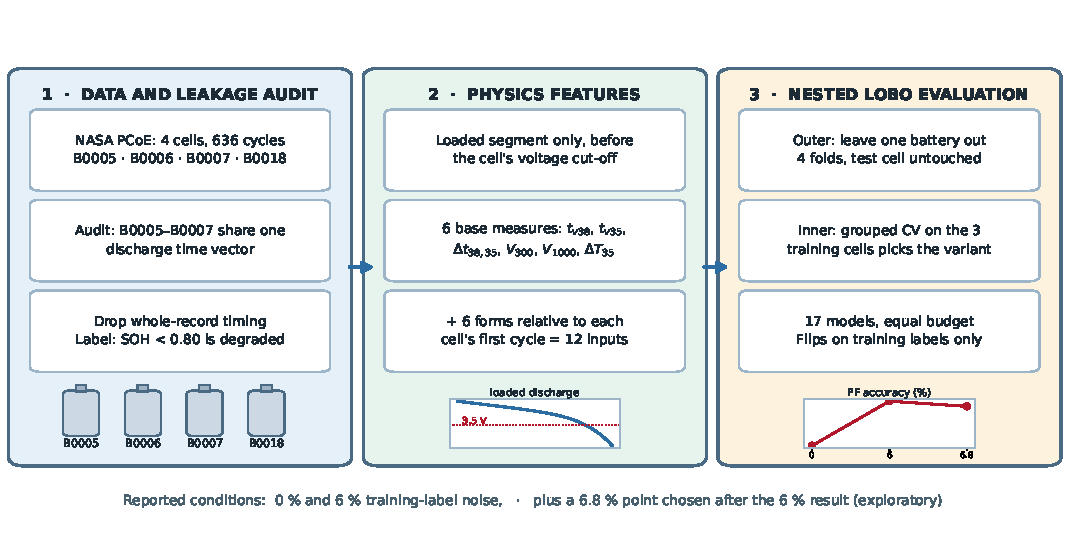
\includegraphics[width=.98\textwidth]{figure1_pipeline.pdf}
\caption{Three-stage workflow. Stage~1 audits the NASA records and fixes the label rule; stage~2 builds twelve loaded-discharge features, half of them referenced to each cell's own first cycle; stage~3 evaluates seventeen models under leave-one-battery-out splitting, with the proposed variant chosen inside the training cells of each fold. The inset in stage~3 shows the proposed model's measured accuracy at the three reported conditions.}\label{fig:pipeline}\end{figure*}

\subsection{NASA dataset, record audit, and features}
We use NASA PCoE cells B0005, B0006, B0007 and B0018, comprising 636 discharge cycles in total\footnote{NASA PCoE battery dataset: \href{https://www.nasa.gov/intelligent-systems-division/discovery-and-systems-health/pcoe/pcoe-data-set-repository/}{NASA Prognostics Data Repository}; dataset coverage is surveyed by Hasib et al.~\cite{hasib2021}.}. SOH is defined as cycle capacity divided by that cell's first-cycle capacity, and a cycle is labelled degraded when SOH $<0.80$. The resulting degraded/healthy counts are 66/102 for B0005, 108/60 for B0006, 45/123 for B0007 and 58/74 for B0018, as listed in Table~\ref{tab:cells}. Two properties of the source records drive the feature design. B0005--B0007 share identical discharge time vectors in every cycle, while B0018 was recorded separately; and whole-record summaries can contain rest intervals governed by another cell's cut-off. Features are therefore computed only on the loaded section that precedes the cell-specific cut-off.

Six measurements are taken from that section: the time from load-on to 3.8\,V and to 3.5\,V, the interval between those two crossings, the terminal voltage at 300\,s and at 1000\,s, and the temperature rise up to the 3.5\,V crossing. Each measurement appears in raw form and in a form relative to the same cell's first cycle --- a ratio for durations, a difference for voltage and temperature --- giving the twelve inputs of Table~\ref{tab:features}. The first cycle is label-free, so a test cell contributes its own reference without contributing a label.
\begin{table}[!t]\centering\scriptsize\caption{NASA cell counts under the SOH $<0.80$ rule.}\label{tab:cells}\begin{tabular}{lrrr}\toprule Cell&Cycles&Degraded&Healthy\\\midrule B0005&168&66&102\\B0006&168&108&60\\B0007&168&45&123\\B0018&132&58&74\\\midrule Total&636&277&359\\\bottomrule\end{tabular}\end{table}
\begin{figure*}[!t]\centering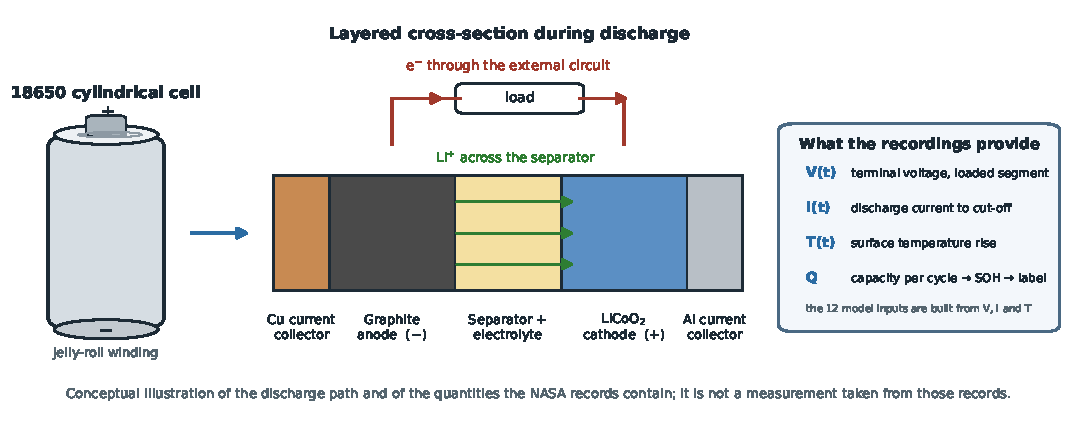
\includegraphics[width=.92\textwidth]{fig12_18650_discharge_schematic.pdf}
\caption{Discharge path of an 18650 cell and the quantities the NASA records contain. Lithium ions move from the graphite anode across the separator to the LiCoO$_2$ cathode while electrons travel through the external load; the recorded voltage, current, temperature and per-cycle capacity are the basis of the twelve features and of the SOH label. The drawing is conceptual and is not a measurement taken from the NASA recordings.}\label{fig:cell-schematic}\end{figure*}
Fig.~\ref{fig:cell-schematic} gives the electrochemical context for those measurements: it shows which physical transport process each recorded signal observes, and where the capacity that defines the label comes from. It is included as explanatory context and is not used to infer any experimental result.

\begin{figure*}[!t]\centering
\begin{subfigure}[t]{.455\textwidth}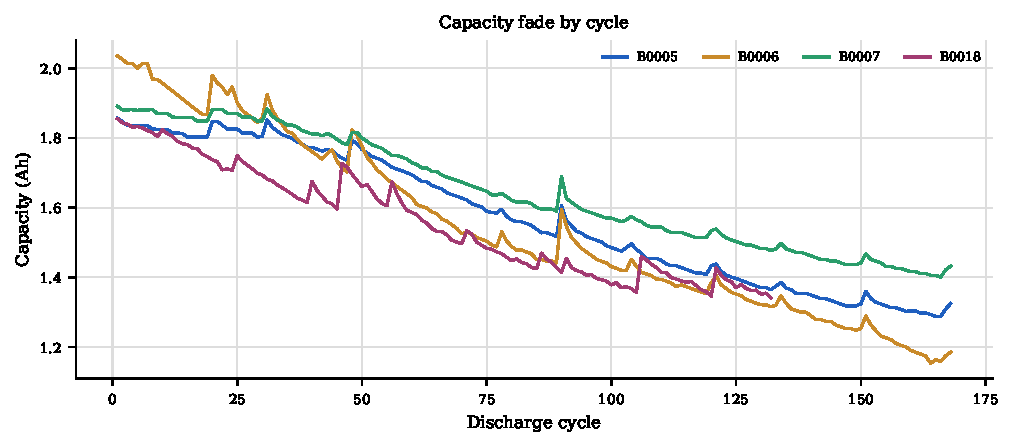
\includegraphics[width=\linewidth]{fig01_capacity_fade.pdf}\caption{Capacity}\end{subfigure}\hfill\begin{subfigure}[t]{.455\textwidth}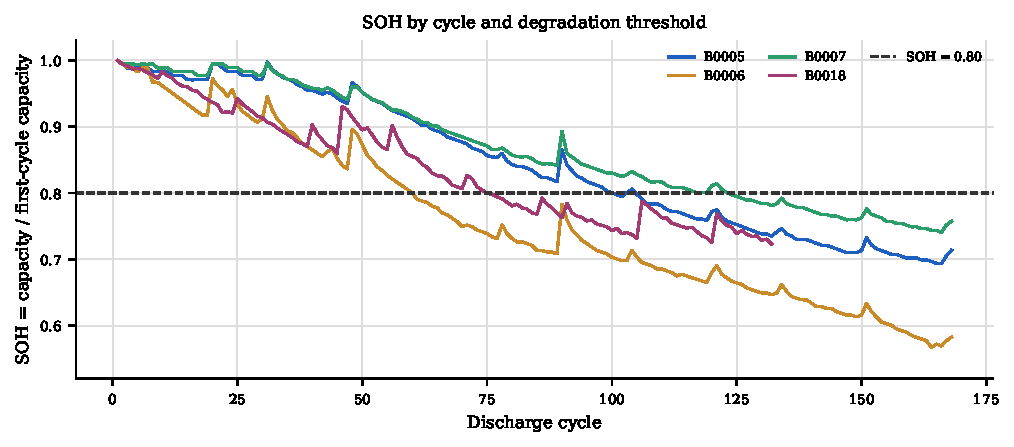
\includegraphics[width=\linewidth]{fig02_soh_threshold.pdf}\caption{SOH threshold}\end{subfigure}\\[1mm]
\begin{subfigure}[t]{.455\textwidth}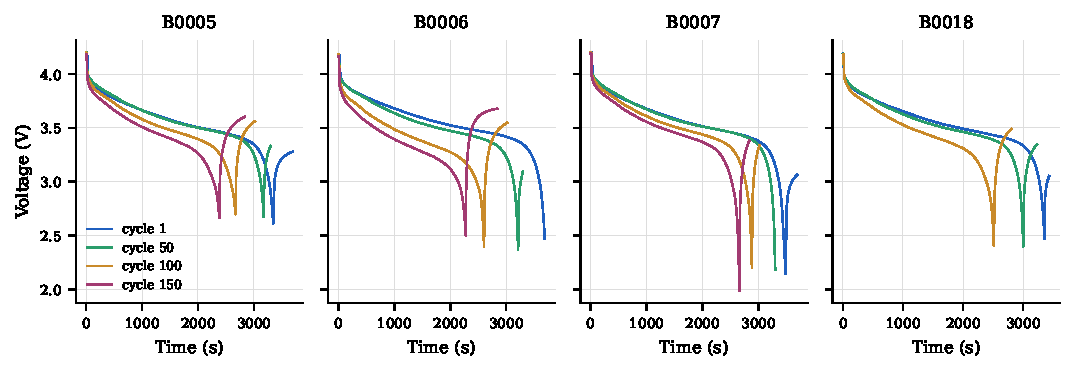
\includegraphics[width=\linewidth]{fig03_voltage_curves.pdf}\caption{Voltage}\end{subfigure}\hfill\begin{subfigure}[t]{.455\textwidth}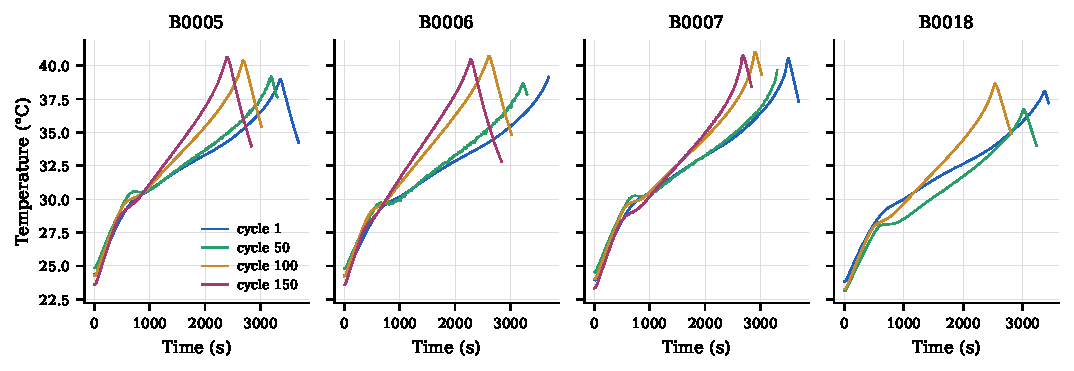
\includegraphics[width=\linewidth]{fig04_temperature_curves.pdf}\caption{Temperature}\end{subfigure}\\[1mm]
\begin{subfigure}[t]{.455\textwidth}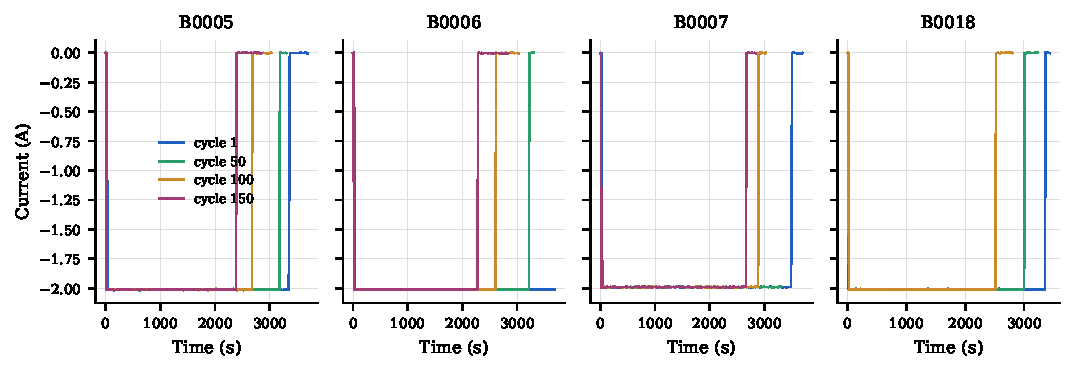
\includegraphics[width=\linewidth]{fig05_current_curves.pdf}\caption{Current}\end{subfigure}\hfill\begin{subfigure}[t]{.455\textwidth}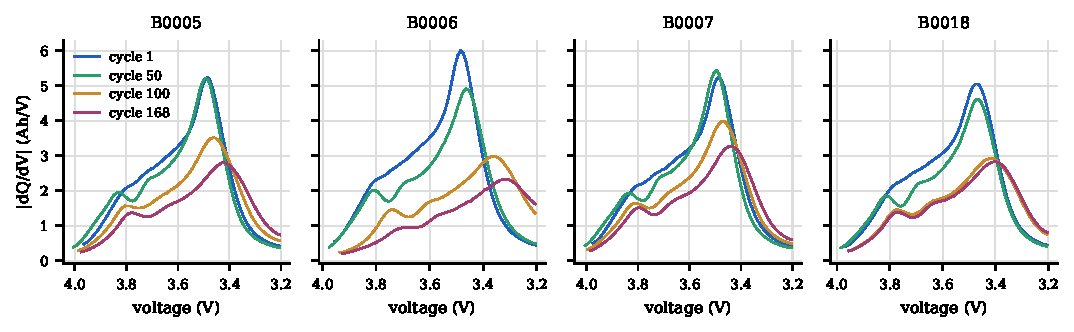
\includegraphics[width=\linewidth]{fig06_incremental_capacity.pdf}\caption{Incremental capacity}\end{subfigure}
\caption{Ageing and loaded-discharge signals for the four cells. Panel~(b) marks the 0.80 SOH line that defines the label. These are raw traces, not noise conditions; the $|dQ/dV|$ view in panel~(f) is diagnostic and is not one of the twelve classifier inputs.}\label{fig:battery-signals}\end{figure*}
Fig.~\ref{fig:battery-signals} shows capacity fade, the SOH threshold, and the voltage, temperature, current and incremental-capacity traces. The four cells cross the 0.80 line at different cycle numbers and with different amounts of local capacity regeneration, which is the main reason the per-cell results in Section~\ref{sec:percell} are heterogeneous. Fig.~\ref{fig:features} shows the feature correlation matrix and the class-conditional distributions. Both remain descriptive, because cycles within a cell are strongly correlated and the effective sample size is closer to four cells than to 636 cycles.
\begin{figure*}[!t]\centering\begin{subfigure}[t]{.465\textwidth}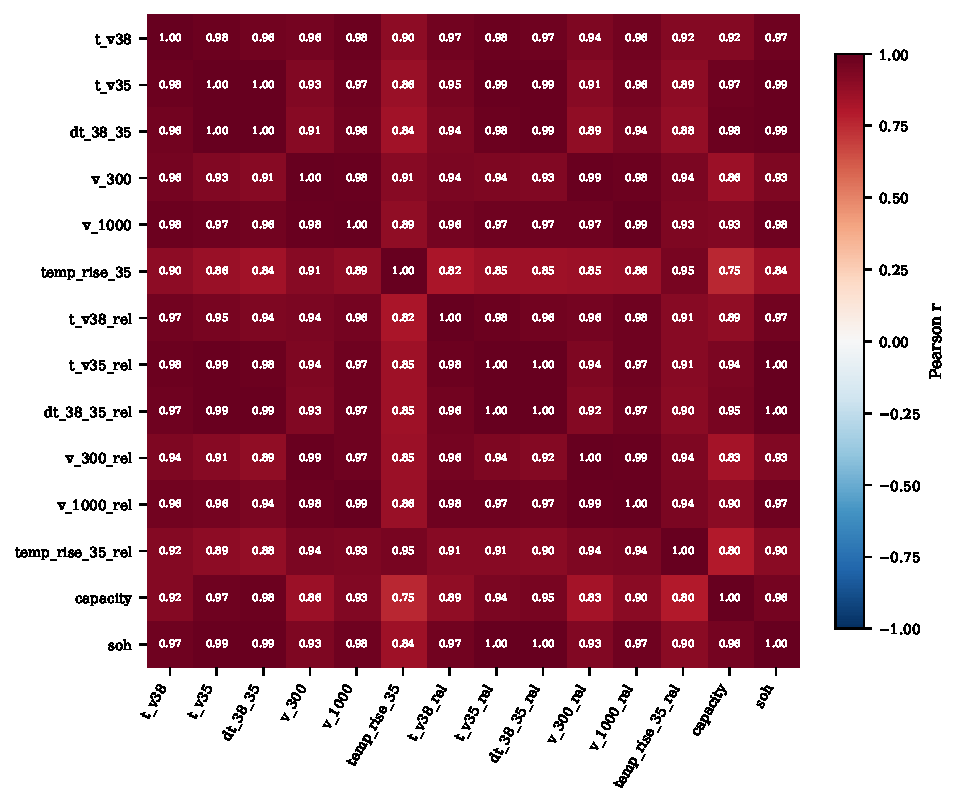
\includegraphics[width=\linewidth]{fig07_feature_correlation.pdf}\caption{Correlation}\end{subfigure}\hfill\begin{subfigure}[t]{.465\textwidth}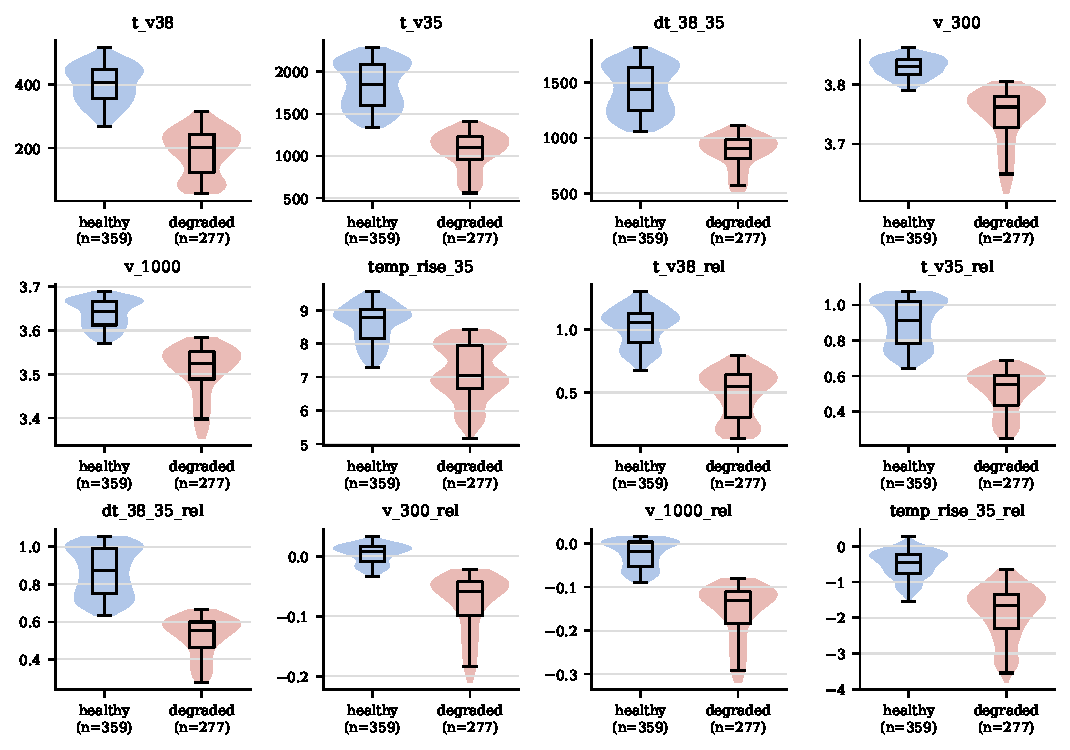
\includegraphics[width=\linewidth]{fig08_feature_distributions.pdf}\caption{Class-conditional distributions}\end{subfigure}\caption{Descriptive analysis of the twelve loaded-discharge features. The relative forms use each cell's own first cycle, so they are comparable across cells without any label information.}\label{fig:features}\end{figure*}
\begin{table}[!t]\centering\scriptsize\caption{The twelve model inputs.}\label{tab:features}\begin{tabularx}{\columnwidth}{lXl}\toprule Base measure&Interpretation&Relative form\\\midrule $t_{v38}$&Time to 3.8 V&Ratio\\$t_{v35}$&Time to 3.5 V&Ratio\\$\Delta t_{38,35}$&Time between thresholds&Ratio\\$V_{300}$&Voltage after 300 s&Difference\\$V_{1000}$&Voltage after 1000 s&Difference\\$\Delta T_{35}$&Temperature rise to 3.5 V&Difference\\\bottomrule\end{tabularx}\par\smallskip{\scriptsize Ratios and differences are taken against the same cell's first, label-free cycle.}\end{table}

\subsection{EF-GBTSVM formulation and variants}\label{sec:formulation}
For training samples $(x_i,y_i)$, a granular ball $GB_j$ is described by its centre $c_j$, majority label $t_j$, size $n_j$ and purity $\pi_j$:
\begin{equation}\begin{aligned}c_j&=\frac{1}{n_j}\sum_{x_s\in GB_j}x_s,\\t_j&=\arg\max_{c\in\{\pm1\}}|\{x_s:y_s=c\}|,\\\pi_j&=\frac{1}{n_j}\max_{c\in\{\pm1\}}|\{x_s:y_s=c\}|.\end{aligned}\end{equation}
Balls whose purity falls below the threshold $\tau$ are split recursively by 2-means. The $k$ surviving centres are stacked into $C\in\mathbb{R}^{k\times m}$. With fixed random weights $W$, bias $b$ and activation $\phi$, the enhanced representation is
\begin{equation}Z=\phi(CW+\mathbf{1}b^\top),\qquad T=[Z,C].\end{equation}
For class matrices $T_1,T_2$ and slack vectors $\xi_1,\xi_2$, the twin-plane primal problems are
\begin{align}\min_{w_1,b_1,\xi_2}\;&\tfrac12\|T_1w_1+e_1b_1\|^2+d_1e_2^\top\xi_2\\\text{s.t. }&-(T_2w_1+e_2b_1)+\xi_2\ge e_2,\quad\xi_2\ge0,\\\min_{w_2,b_2,\xi_1}\;&\tfrac12\|T_2w_2+e_2b_2\|^2+d_2e_1^\top\xi_1\\\text{s.t. }&(T_1w_2+e_1b_2)+\xi_1\ge e_1,\quad\xi_1\ge0.\end{align}
With $F=[T_1\ e_1]$, $E=[T_2\ e_2]$ and ridge $\delta>0$, the duals are
\begin{align}\max_{0\le\alpha\le d_1e_2}\;&e_2^\top\alpha-\tfrac12\alpha^\top E(F^\top F+\delta I)^{-1}E^\top\alpha,\\\max_{0\le\gamma\le d_2e_1}\;&e_1^\top\gamma-\tfrac12\gamma^\top F(E^\top E+\delta I)^{-1}F^\top\gamma,\end{align}
and the planes and decision rule follow as
\begin{equation}\begin{aligned}\begin{bmatrix}w_1\\b_1\end{bmatrix}&=-(F^\top F+\delta I)^{-1}E^\top\alpha,\\\begin{bmatrix}w_2\\b_2\end{bmatrix}&=(E^\top E+\delta I)^{-1}F^\top\gamma,\\\hat y(x)&=\arg\min_{i\in\{1,2\}}\frac{|w_i^\top\psi(x)+b_i|}{\|w_i\|},\end{aligned}\end{equation}
with $\psi(x)=[\phi(xW+b^\top),x]$.

Our implementation differs from the published description in ways that should be stated plainly, because they affect reproducibility: standardisation is fitted on training data only; small balls are dropped unless doing so would remove a class entirely; 2-means uses three seeded starts with a fallback for degenerate splits; $W\sim U[-1,1]$, $b\sim 0.1\,U[0,1]$ and $\delta=0.05$; the candidate grids use eight values of $d$ between $10^{-5}$ and $10^{2}$, five hidden sizes and five activations including an added hyperbolic tangent; and the GBTSVM ablation omits the original radius terms. These describe our reimplementation, not the authors' code.

Table~\ref{tab:variants} lists the controlled variants and structural ablations. The per-fold selector considers five candidates --- EF-GBTSVM, L8, J, M and JM --- and ranks them by mean inner-validation balanced accuracy on the three training cells before refitting. The recorded selections were L8 when B0005, B0007 or B0018 was held out, and J when B0006 was held out.
\begin{table*}[!t]\centering\scriptsize\caption{Controlled variants and structural ablations. The first group changes how balls are formed; the second removes a structural component.}\label{tab:variants}\begin{tabularx}{\textwidth}{l l X}\toprule Entry&Representation&Definition\\\midrule EF-GBTSVM&balls + enhanced&Reference purity grid\\EF-GBTSVM-W&balls + enhanced&Wide purity grid; purity-weighted bounds\\EF-GBTSVM-L&balls + enhanced&Wide fixed purity grid\\EF-GBTSVM-A&balls + enhanced&$k$NN-error purity heuristic\\EF-GBTSVM-L8&balls + enhanced&Eight-value purity grid\\EF-GBTSVM-J&balls + enhanced&$k$NN-error rule with offset search\\EF-GBTSVM-M/JM&weighted balls&Mass weighting; JM combines J with weighting\\\proposed&balls + enhanced&Per-fold inner-CV selection among five variants\\\midrule GBTSVM&balls + original&No enhanced map; radius-term deviation noted\\HF-GBTSVM&balls + hidden&Hidden features only\\EF-TSVM&no balls + enhanced&Sample-level enhanced twin SVM\\TSVM&no balls + original&Original features\\\bottomrule\end{tabularx}\end{table*}
\begin{figure*}[!t]\centering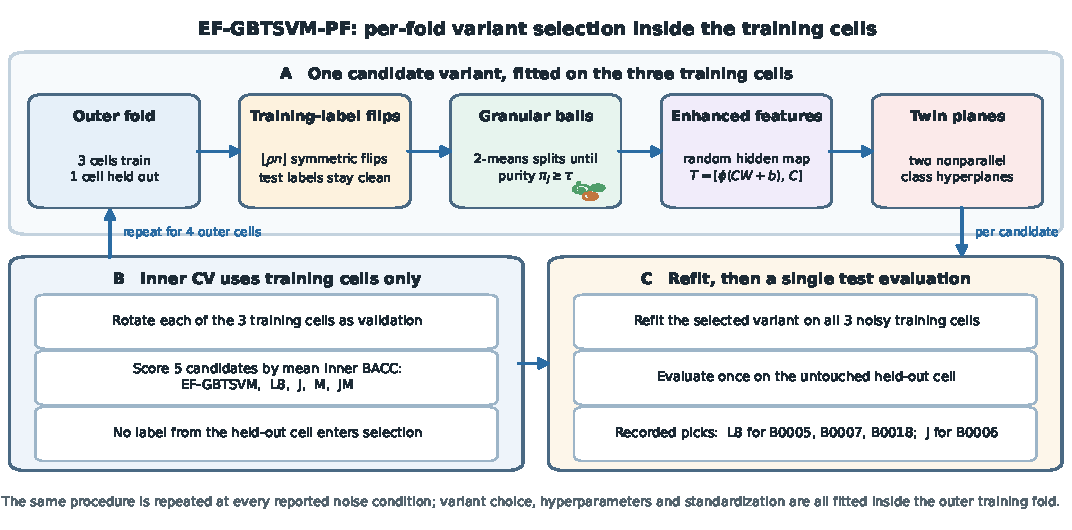
\includegraphics[width=.99\textwidth]{figure5_pf_nested_cv.pdf}
\caption{Architecture of \proposed\ and its per-fold selection. Panel~A is the pipeline followed by one candidate variant; panel~B shows the inner cross-validation, which rotates the three training cells and never uses a held-out label; panel~C refits the selected variant and evaluates it once on the untouched cell.}\label{fig:pf}\end{figure*}
\noindent\fbox{\begin{minipage}{0.955\columnwidth}\textbf{Algorithm 1. Nested LOBO procedure for \proposed.}\par\smallskip\textbf{Input:} four cells; candidate variants EF, L8, J, M, JM; noise rate $\rho$.\par\textbf{For each outer test cell:} (1) hold out all of its cycles; (2) inject the prescribed exact-count symmetric flips into the other three cells only; (3) rotate each training cell as inner validation and compute the mean balanced accuracy of each candidate; (4) select the candidate from those inner results, refit it on all three training cells, and evaluate once on the untouched outer cell.\par\textbf{Output:} one outer-fold prediction set and one selected variant per noise condition.\end{minipage}}
\par\smallskip
Fig.~\ref{fig:balls} shows a two-dimensional PCA view of the resulting balls and the measured relationship between the purity threshold and the number of balls. The PCA view is for visualisation only; training takes place in the original standardised space. A higher purity threshold forces more splits, as expected, but this diagnostic on its own does not demonstrate a predictive benefit.
\begin{figure*}[!t]\centering\begin{subfigure}[t]{.49\textwidth}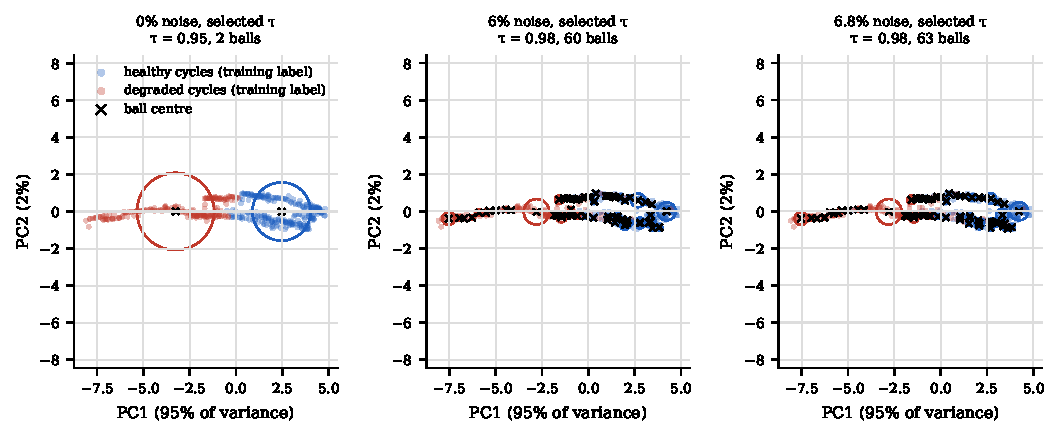
\includegraphics[width=\linewidth]{fig10_granular_balls_pca.pdf}\caption{PCA view of the balls}\end{subfigure}\hfill\begin{subfigure}[t]{.49\textwidth}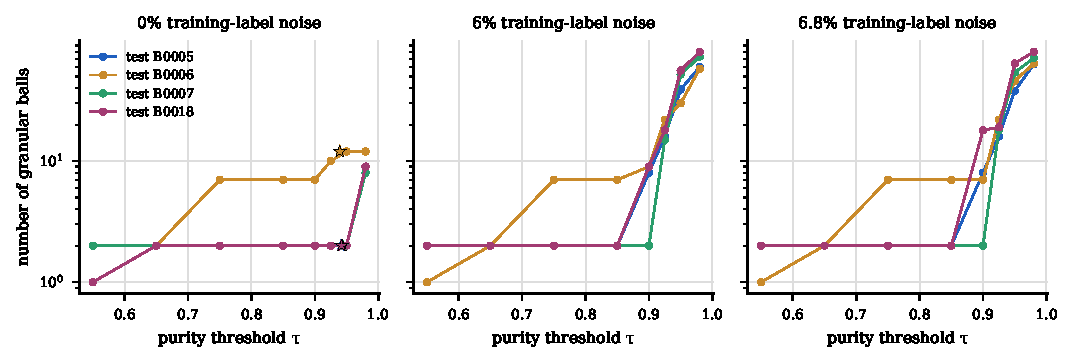
\includegraphics[width=\linewidth]{fig11_balls_vs_purity.pdf}\caption{Ball count against $\tau$}\end{subfigure}\caption{Granular-ball diagnostics at the three reported noise conditions. Raising the purity threshold forces more splits, as expected; on its own this does not demonstrate a predictive benefit.}\label{fig:balls}\end{figure*}

\subsection{Experimental protocol and equal tuning budget}\label{sec:protocol}
Outer evaluation leaves one battery out, so training uses 468 cycles, or 504 when B0018 is the held-out cell. Exact-count symmetric noise flips $\lfloor\rho n\rfloor$ training labels using seed $1000+\text{fold}$; every model in a given fold receives exactly the same flipped labels, and test labels are never altered. Standardisation is fitted inside the training pipeline. Randomised hyperparameter search evaluates $\min(150,|\mathcal{G}|)$ candidates per model using three battery-grouped inner folds with balanced-accuracy selection, which equalises the search budget across models of very different grid sizes (Table~\ref{tab:search}).

Two of the three reported conditions were fixed before being run: 0\nz, which leaves the training labels untouched, and 6\nz. The third, 6.8\nz, was run only after the 6\nz\ result had been observed, on the same four cells and the same features. Choosing where to look after seeing an outcome inflates the chance of finding a further favourable point in that neighbourhood, so this condition carries less evidential weight than one fixed in advance; it is identified as exploratory throughout, and Section~\ref{sec:limits} returns to it.

\subsection{Evaluation metrics and software}
For confusion counts $TP,TN,FP,FN$ the reported metrics are
\begin{align}\mathrm{ACC}&=\frac{TP+TN}{TP+TN+FP+FN},\\\mathrm{BACC}&=\tfrac12\left(\frac{TP}{TP+FN}+\frac{TN}{TN+FP}\right),\\\mathrm{F1}&=\frac{2TP}{2TP+FP+FN},\qquad\mathrm{AUC}=\int_0^1\mathrm{TPR}(u)\,du.\end{align}
Balanced accuracy is the primary selection criterion because the class ratio differs substantially between cells. We report the mean and standard deviation over the four held-out cells, together with the rank among the seventeen models shown. Two of those seventeen, EF-GBTSVM-L8 and EF-GBTSVM-J, are marked with a dagger: they are the candidates from which \proposed\ is assembled, so they are shown for completeness but were outside the pre-registered fifteen-model comparison pool. The recorded software stack is Python 3.13.9, scikit-learn 1.8.0, SciPy 1.15.3, NumPy 2.2.6, pandas 2.3.3, XGBoost 3.1.3 and CVXOPT 1.3.3.
\begin{table}[!t]\centering\scriptsize\caption{Search spaces and grid sizes; randomised search is capped at 150 candidates per model.}\label{tab:search}\begin{tabularx}{\columnwidth}{lXr}\toprule Model&Search dimensions&Size\\\midrule EF-GBTSVM/W/L/HF&$d$:8, hidden:5, activation:5, $\tau$:5&1000\\L8&$d$:8, hidden:5, activation:5, $\tau$:8&1600\\J&$d$:8, hidden:5, activation:5, offset:5&1000\\A/EF-TSVM&$d$:8, hidden:5, activation:5&200\\GBTSVM&$d$:8, $\tau$:5&40\\TSVM&$d$:8&8\\RVFL&$C$:8, hidden:5, activation:5&200\\RBF-SVM&$C$:10, $\gamma$:15&150\\Random forest&trees:4, depth:5, leaf:4, features:3&240\\MLP&hidden:6, L2:7, rate:2, activation:2&168\\XGBoost&trees:4, depth:5, rate:4, subsample:2&160\\\bottomrule\end{tabularx}\end{table}

\section{Results and discussion}\label{sec:results}
\subsection{Overall benchmark}
Table~\ref{tab:main} gives the mean accuracy and balanced accuracy of all seventeen models at the three reported conditions, each with its rank among the seventeen; the shaded row marks the proposed model. The result is narrow and specific. On clean labels \proposed\ reaches 95.25\nz\ accuracy and ranks twelfth of seventeen. Eleven models are ahead of it: TSVM at 98.77\nz, RVFL at 97.75\nz, XGBoost at 97.69\nz, MLP at 97.61\nz, random forest at 97.39\nz, EF-GBTSVM-J at 97.21\nz, the single-feature threshold at 96.94\nz, EF-TSVM at 96.67\nz, HF-GBTSVM at 96.47\nz, GBTSVM at 96.43\nz\ and EF-GBTSVM-A at 95.73\nz. Nothing in the clean-label result can therefore be credited to granular-ball aggregation: a one-feature decision stump and three of our own ablations all do better. At 6\nz\ training-label noise it reaches 98.01\nz\ accuracy and 98.10\nz\ balanced accuracy, first of seventeen on both. At the exploratory 6.8\nz\ point it reaches 97.69\nz\ and 97.67\nz, again first on both.
\begin{table*}[!t]\centering\scriptsize\setlength{\tabcolsep}{5.5pt}
\caption{Mean test accuracy and balanced accuracy (\%) $\pm$ standard deviation over the four held-out cells, with the rank among the seventeen models in parentheses (1 = best). All seventeen models are shown; shading marks the proposed selector, and $^{\dagger}$ marks the two candidate variants from which it is assembled. The 6.8\nz\ condition was chosen after the 6\nz\ result and is exploratory.}\label{tab:main}
\begin{tabular}{l*{6}{c}}
\toprule
&\multicolumn{2}{c}{0\%}&\multicolumn{2}{c}{6\%}&\multicolumn{2}{c}{6.8\%}\\
\cmidrule(lr){2-3}\cmidrule(lr){4-5}\cmidrule(lr){6-7}
Model & ACC & BACC & ACC & BACC & ACC & BACC \\
\midrule
EF-GBTSVM & 94.83$\pm$3.68 (16) & 94.97$\pm$3.18 (14) & 97.42$\pm$1.46 (6) & 97.67$\pm$1.30 (4) & 97.12$\pm$3.29 (5) & 96.67$\pm$3.98 (4) \\
EF-GBTSVM-A & 95.73$\pm$2.47 (11) & 94.56$\pm$2.90 (15) & 94.95$\pm$2.85 (11) & 94.82$\pm$2.26 (10) & 94.24$\pm$3.02 (12) & 94.11$\pm$2.30 (13) \\
EF-GBTSVM-L & 95.25$\pm$3.11 (12) & 95.24$\pm$2.45 (10) & 93.76$\pm$3.46 (13) & 90.84$\pm$7.70 (13) & 93.52$\pm$9.99 (13) & 95.10$\pm$6.56 (9) \\
EF-GBTSVM-W & 95.25$\pm$3.11 (12) & 95.24$\pm$2.45 (10) & 93.76$\pm$3.46 (13) & 90.84$\pm$7.70 (13) & 93.52$\pm$9.99 (13) & 95.10$\pm$6.56 (9) \\
EF-GBTSVM-L8$^{\dagger}$ & 95.10$\pm$2.97 (15) & 95.03$\pm$2.32 (13) & 97.71$\pm$1.77 (4) & 97.87$\pm$1.76 (2) & 97.24$\pm$1.31 (4) & 97.05$\pm$1.95 (2) \\
EF-GBTSVM-J$^{\dagger}$ & 97.21$\pm$3.34 (6) & 97.23$\pm$3.00 (3) & 97.61$\pm$1.29 (5) & 97.84$\pm$1.16 (3) & 96.92$\pm$3.23 (7) & 96.94$\pm$2.79 (3) \\
\cellcolor{proposedrow}\textbf{EF-GBTSVM-PF (proposed)} & \cellcolor{proposedrow}\textbf{95.25$\pm$3.11 (12)} & \cellcolor{proposedrow}\textbf{95.24$\pm$2.45 (10)} & \cellcolor{proposedrow}\textbf{98.01$\pm$1.97 (1)} & \cellcolor{proposedrow}\textbf{98.10$\pm$1.94 (1)} & \cellcolor{proposedrow}\textbf{97.69$\pm$1.24 (1)} & \cellcolor{proposedrow}\textbf{97.67$\pm$1.40 (1)} \\
GBTSVM & 96.43$\pm$2.53 (10) & 94.44$\pm$4.54 (16) & 94.12$\pm$8.21 (12) & 93.31$\pm$9.37 (12) & 91.37$\pm$5.51 (15) & 90.31$\pm$6.65 (15) \\
HF-GBTSVM & 96.47$\pm$2.92 (9) & 95.76$\pm$2.72 (7) & 96.52$\pm$1.03 (8) & 95.53$\pm$1.48 (8) & 95.78$\pm$5.45 (9) & 94.90$\pm$6.13 (11) \\
EF-TSVM & 96.67$\pm$1.16 (8) & 95.34$\pm$2.83 (9) & 91.13$\pm$9.04 (15) & 89.87$\pm$11.16 (16) & 95.44$\pm$1.96 (10) & 94.71$\pm$2.15 (12) \\
TSVM & 98.77$\pm$0.81 (1) & 98.67$\pm$0.89 (1) & 95.63$\pm$4.21 (9) & 94.83$\pm$5.79 (9) & 91.10$\pm$11.95 (16) & 88.01$\pm$17.02 (16) \\
RBF-SVM & 86.61$\pm$23.25 (17) & 88.29$\pm$17.83 (17) & 89.68$\pm$14.97 (17) & 90.53$\pm$11.74 (15) & 97.27$\pm$0.86 (3) & 96.50$\pm$1.09 (6) \\
RVFL & 97.75$\pm$0.59 (2) & 97.45$\pm$0.97 (2) & 90.08$\pm$10.63 (16) & 89.45$\pm$8.07 (17) & 88.89$\pm$11.64 (17) & 87.79$\pm$9.63 (17) \\
Random forest & 97.39$\pm$1.48 (5) & 96.15$\pm$3.46 (6) & 97.84$\pm$0.95 (2) & 96.91$\pm$2.42 (5) & 97.61$\pm$1.10 (2) & 96.60$\pm$2.40 (5) \\
MLP & 97.61$\pm$0.70 (4) & 96.62$\pm$1.57 (5) & 97.84$\pm$1.52 (2) & 96.66$\pm$3.09 (6) & 97.09$\pm$1.75 (6) & 95.56$\pm$3.78 (8) \\
XGBoost & 97.69$\pm$0.91 (3) & 96.70$\pm$2.39 (4) & 97.09$\pm$1.19 (7) & 95.94$\pm$2.08 (7) & 96.86$\pm$0.57 (8) & 95.64$\pm$1.56 (7) \\
Single-feature threshold & 96.94$\pm$1.97 (7) & 95.47$\pm$4.44 (8) & 95.60$\pm$3.65 (10) & 94.49$\pm$4.07 (11) & 95.16$\pm$3.52 (11) & 93.65$\pm$4.41 (14) \\
\bottomrule
\end{tabular}
\end{table*}

Two cautions apply to every row. First, the standard deviations are large next to the differences between models --- commonly two to six percentage points over four cells, and far more for the least stable baselines --- so a gap of one or two points between adjacent ranks is not a meaningful separation. Second, several baselines are unstable rather than uniformly weak: RBF-SVM carries a standard deviation of 23.25 points at 0\nz\ and is last of seventeen there, yet it is third at 6.8\nz\ with 97.27\nz. A single collapsing fold, not a consistent deficit, produces that pattern.

\subsection{Noise response and rank stability}
Fig.~\ref{fig:mainsweep} presents the same two measures as heatmaps with ranks, which makes the instability of the ordering visible. Three groups emerge. Some models fall steeply as labels are corrupted: TSVM goes from 98.77\nz\ to 95.63\nz\ to 91.10\nz, moving from first to ninth to sixteenth, and RVFL from 97.75\nz\ to 90.08\nz\ to 88.89\nz, from second to last. Others barely move: random forest stays between 97.39 and 97.84\nz\ and MLP between 97.09 and 97.84\nz\ across all three conditions. One moves the other way, RBF-SVM climbing from 86.61\nz\ to 97.27\nz. The granular-ball family is itself split: plain EF-GBTSVM improves from 94.83\nz\ to 97.42\nz\ and 97.12\nz, while the fixed wide-purity variants L and W fall from 95.25\nz\ to 93.76\nz\ and 93.52\nz.
\begin{figure*}[!t]\centering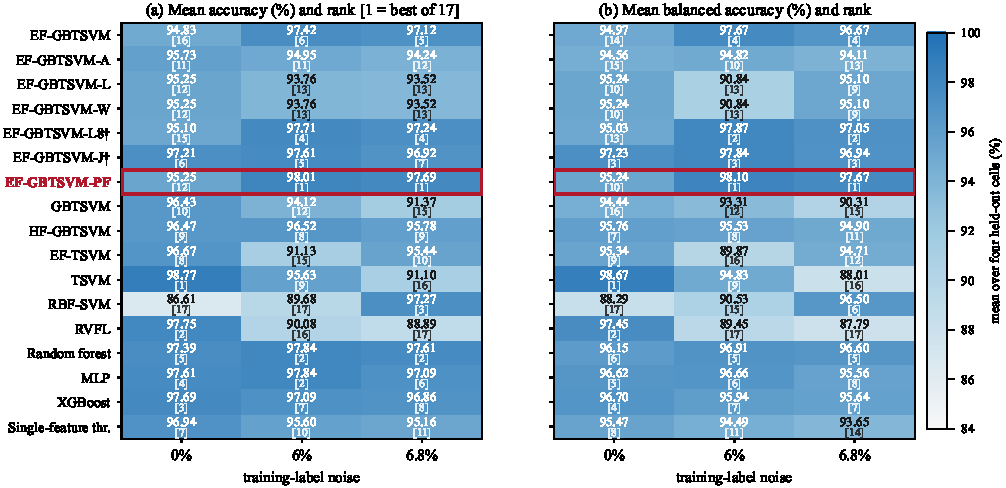
\includegraphics[width=.99\textwidth]{figR1_main_sweep.pdf}
\caption{Accuracy and balanced accuracy of all seventeen models at the three reported conditions, with the rank of each cell printed in brackets. The proposed selector is outlined. There is no common degradation pattern: the ordering of the models changes substantially from one condition to the next.}\label{fig:mainsweep}\end{figure*}

Fig.~\ref{fig:pfvsbest} isolates the practical question --- how far the proposed model sits from the best model available at each condition. The gap is 3.52 points on clean labels, where TSVM leads, and closes to zero at both noisy conditions, where \proposed\ is itself the best. That is the whole of the positive result, and it rests on two conditions measured over four related cells.
\begin{figure}[!htb]\centering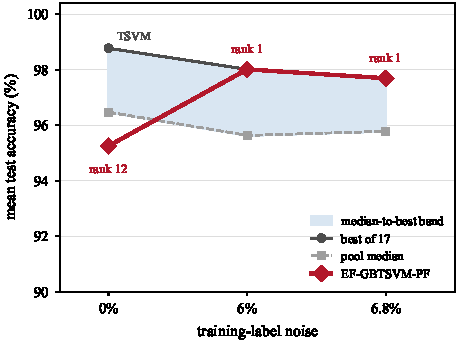
\includegraphics[width=\columnwidth]{figR2_pf_vs_best.pdf}
\caption{Mean accuracy of \proposed\ against the best and the median of the seventeen-model pool at each reported condition. The annotation beside each point is the proposed model's rank there.}\label{fig:pfvsbest}\end{figure}

No significance claim accompanies these ranks, and none is available. Each condition supplies four paired observations, one per held-out cell, so the smallest two-sided $p$-value a paired rank test can attain at a single condition is $0.125$ --- above any conventional threshold before a single comparison is made, and before any correction for comparing seventeen models. Pooling the conditions would not help, because all three reuse the same four cells and the same features, so the observations are not independent. The ranks in Table~\ref{tab:main} are descriptive summaries of these four cells, and the design is underpowered to detect differences of the size observed.

The 6.8\nz\ condition also carries less weight than the other two. It was run after the 6\nz\ result had been seen, on the same cells, so it re-examines that observation rather than testing it afresh. Two of the three reported conditions are therefore not independent of one another, which is the main reason the ranks here should not be read as a general property of the method.

\subsection{Per-battery behaviour}\label{sec:percell}
Fig.~\ref{fig:percell} shows the four held-out cells separately at each reported condition. The spread between cells is wider than the spread between most models, which is the central caution of this study. A single misclassified cycle changes accuracy by 0.60 points for B0005--B0007 and by 0.76 points for B0018, so the differences that separate neighbouring ranks correspond to a handful of cycles. B0006 is consistently the hardest fold: it has the most degraded cycles (108 of 168) and is the cell for which the selector chose the J variant rather than L8.
\begin{figure*}[!t]\centering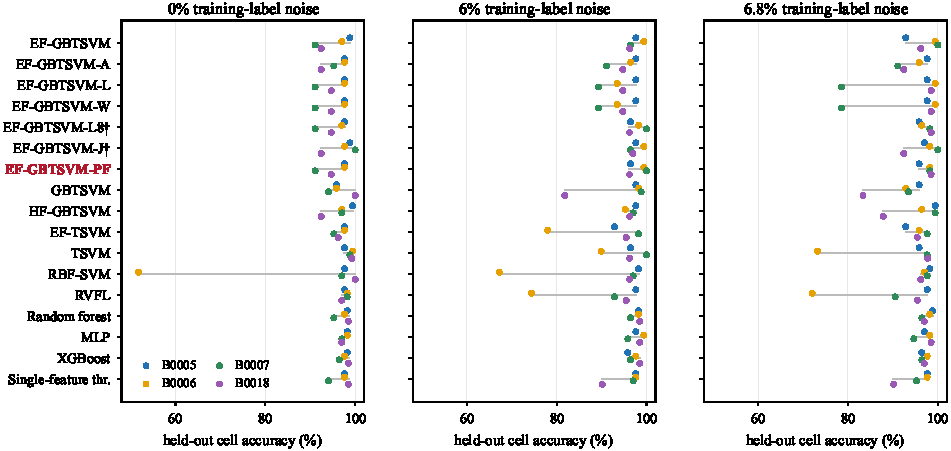
\includegraphics[width=.99\textwidth]{figR5_per_cell.pdf}
\caption{Accuracy on each held-out cell. Each point is one outer fold, and the grey bar spans the four cells for that model. The four points are held-out batteries from one dataset, not independent random replicates, so the spread describes these four cells and is not an estimate of fleet-wide variation.}\label{fig:percell}\end{figure*}

\subsection{Ablation analysis}\label{sec:ablation}
The ablations in Table~\ref{tab:variants} separate the contributions of the two structural components. Removing the enhanced mapping while keeping the balls gives GBTSVM, and removing the balls while keeping the mapping gives EF-TSVM; removing both gives plain TSVM. At 0\nz\ plain TSVM is the single best model in the pool at 98.77\nz, so neither component earns its place on clean labels. Under noise the two separate. GBTSVM, which keeps the balls and drops the enhanced mapping, falls from 96.43\nz\ to 94.12\nz\ and then 91.37\nz. EF-TSVM, which keeps the mapping and drops the balls, falls from 96.67\nz\ to 91.13\nz\ at 6\nz. Only the full combination improves as labels are corrupted: EF-GBTSVM rises from 94.83\nz\ to 97.42\nz\ and 97.12\nz. Neither component on its own reproduces that behaviour here, which is suggestive, but with four cells and three conditions the comparison cannot isolate a causal mechanism.

The per-fold selector contributes through variant choice rather than through a new learning rule. Its selections vary across held-out cells --- L8 for three folds and J for one --- and it therefore tracks whichever fixed variant happens to suit a fold, which is why it is usually better than the worst fixed variant and rarely better than the best. The single-feature threshold baseline, tuned under the same protocol, is a useful reference point: it reaches 96.94\nz\ on clean labels --- ahead of the proposed model --- and 95.60\nz\ and 95.16\nz\ at the two noisy conditions, which bounds how much any of the learned models actually add on this data.

\subsection{Error analysis, ROC, sensitivity and runtime}
Saved prediction records were retained only at 0\nz, so the pooled confusion analysis is restricted to that condition. At 0\nz, \proposed\ produces 335 correctly classified healthy cycles, 24 healthy cycles predicted as degraded, 6 degraded cycles predicted as healthy and 271 correctly classified degraded cycles, giving 30 errors in total (Fig.~\ref{fig:confusion}). The errors are asymmetric in the direction a BMS would prefer: four times as many healthy cycles are flagged as degraded as degraded cycles are missed. That asymmetry should be read alongside the fold class counts and does not imply the same behaviour at noisy conditions.
\begin{figure*}[!t]\centering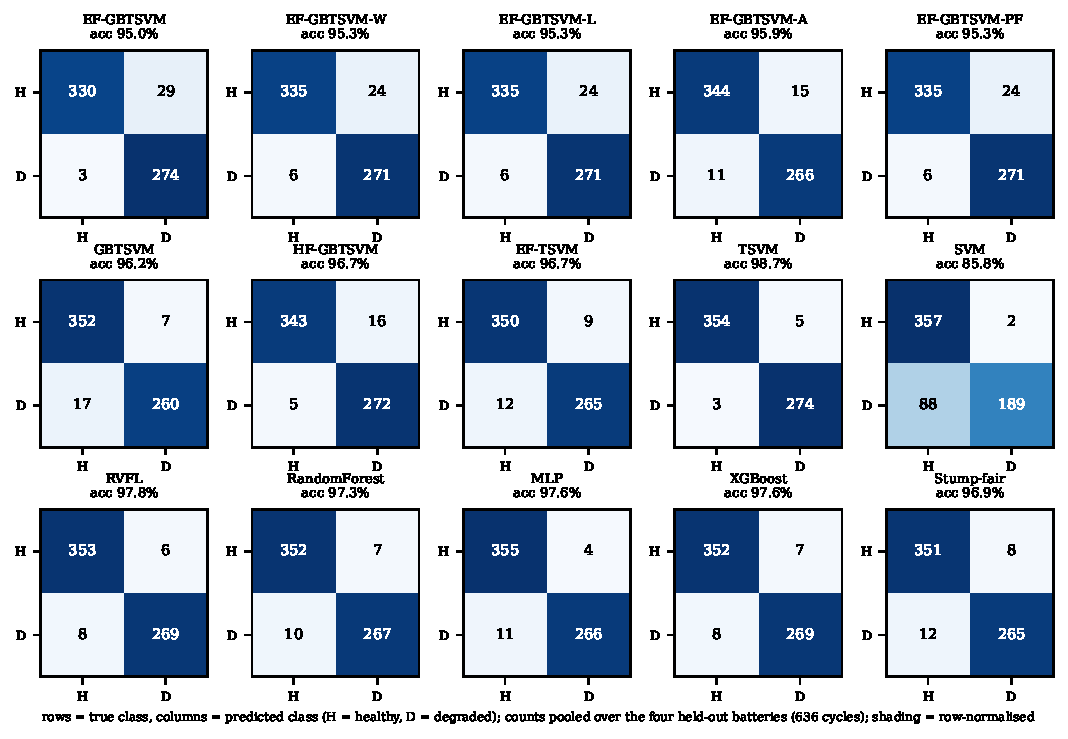
\includegraphics[width=.98\textwidth]{fig18_confusion_matrices_noise0.pdf}
\caption{Pooled confusion matrices at 0\nz\ noise, the only condition for which the per-cycle predictions were saved. Counts are pooled over the four held-out cells (636 cycles); pooling is descriptive and does not remove the dependence among cycles from the same battery.}\label{fig:confusion}\end{figure*}
\begin{figure*}[!t]\centering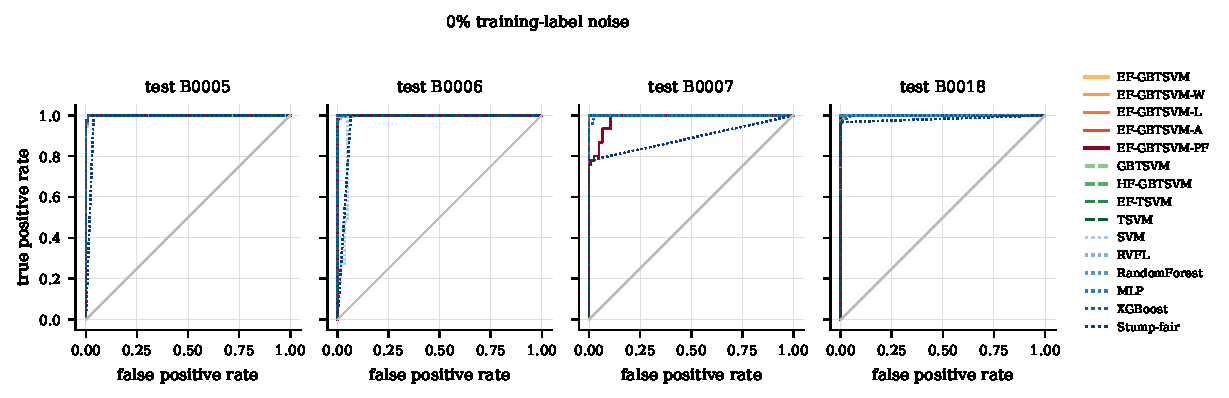
\includegraphics[width=.99\textwidth]{fig19_roc_curves_noise0.pdf}
\caption{Per-cell ROC curves at 0\nz\ noise, one panel per held-out battery, for all models whose prediction scores were saved.}\label{fig:roc}\end{figure*}
Fig.~\ref{fig:roc} shows the per-cell ROC curves at the same condition. \proposed\ has a mean AUC of 99.59\nz\ with a standard deviation of 0.75 points over the four held-out cells, and the curves for most models lie close to the upper-left corner on three of the four cells. B0007 is the exception: several models show a visible shoulder there, which is the fold with the fewest degraded cycles (45 of 168) and therefore the one where a few misranked cycles move the curve most. The ranking these models produce is therefore good even where their thresholded accuracy is not, so part of the accuracy spread in Table~\ref{tab:main} reflects where the decision boundary falls rather than how well the cycles are ordered. ROC curves do not select that operating point, and because scores were saved only at 0\nz\ no noisy-condition comparison of this kind is possible.
\begin{figure*}[!t]\centering
\begin{subfigure}[t]{.49\textwidth}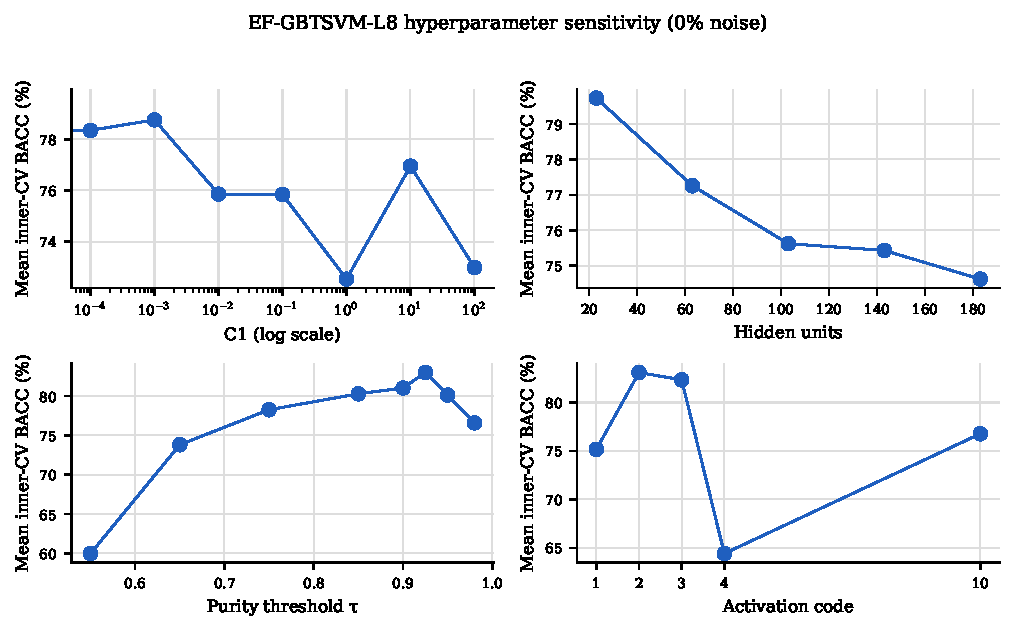
\includegraphics[width=\linewidth]{fig21_hyperparameter_sensitivity_noise0.pdf}\caption{Inner-fold sensitivity traces for the EF-GBTSVM-L8 variant: mean inner-validation balanced accuracy against the regularisation parameter, the number of hidden units, the purity threshold $\tau$, and the activation code.}\label{fig:sensitivity}\end{subfigure}\hfill
\begin{subfigure}[t]{.49\textwidth}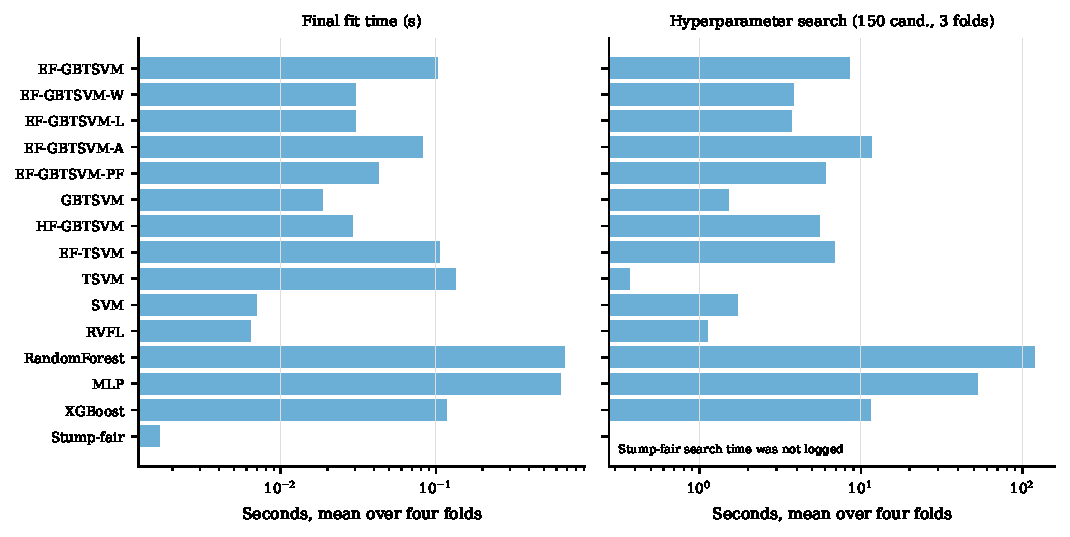
\includegraphics[width=\linewidth]{fig20_runtime_noise0.pdf}\caption{Recorded wall-clock time: final fit time (left) and total hyperparameter-search time over 150 candidates and three inner folds (right), each a mean over the four outer folds.}\label{fig:runtime}\end{subfigure}
\caption{Tuning and timing diagnostics at 0\nz\ noise, the condition for which these records were retained.}\label{fig:diagnostics}\end{figure*}
Fig.~\ref{fig:sensitivity} reports what the inner validation actually saw while tuning. The purity trace rises across most of its range and peaks locally near $\tau=0.925$, which is consistent with the ball-count behaviour in Fig.~\ref{fig:balls}: more aggressive splitting helps until the balls become small enough to behave like individual samples. The hidden-unit trace runs the other way and is strongest at the smallest size tested, which suggests the enhanced mapping is not the component doing the work on this data and agrees with the ablation result of Section~\ref{sec:ablation}. The regularisation and activation traces are non-monotone. These are inner-validation scores on training cells, not independent test estimates, so they show what the selector preferred here, not a universal optimum.
Fig.~\ref{fig:runtime} separates fit cost from search cost, which matters because the two differ by orders of magnitude. Granular-ball final fits complete in hundredths of a second in the logged run, since the twin planes are solved over a few hundred ball centres rather than over 468 or 504 cycles, whereas some conventional searches take tens of seconds. A deployed classifier pays the fit cost, not the search cost, so this family is cheap to retrain once its hyperparameters are fixed. These machine-specific records establish nothing about embedded latency, memory or energy, which need measurement on target hardware.

A train-versus-test gap check was run by refitting with the logged best parameters on the same training fold: the refit reproduces the logged test accuracy exactly on all 180 recorded rows, and on clean labels the gap between training accuracy on true labels and test accuracy is 1.48 points for \proposed. The proposed model is therefore not overfitting its training folds; its limitations are in generalisation across cells, not in memorisation.

\subsection{Positioning against recent SOH literature}\label{sec:lit}
Table~\ref{tab:sota} compares this study with the three recent works introduced in Section~\ref{sec:related} on task, data, evaluation design and metric family. Their figures are reproduced in their own units and are not placed in a shared column with our accuracies, because the two metric families answer different questions: RMSE measures the magnitude of a continuous SOH prediction error, while accuracy and balanced accuracy measure thresholded class decisions. A low regression RMSE does not fix the sensitivity or specificity of a decision at SOH 0.80 without an explicit prediction-to-classification rule applied to cycle-level predictions.
\begin{table*}[!t]\centering\scriptsize\caption{Comparison with three recent SOH studies. Metrics are reproduced in the units each source reports and are not comparable across rows; no claim is made that the present model outperforms any of them.}\label{tab:sota}
\begin{tabularx}{\textwidth}{>{\raggedright\arraybackslash}p{2.0cm} >{\raggedright\arraybackslash}p{2.9cm} X X}\toprule
Study&Task and data&Evaluation as reported&Reported metrics, in the source's own scale\\\midrule
Xu et al.~\cite{xu2026}&SOH regression; NASA B0005--B0007 and MIT cells; dynamic-kernel sparse variational GP&Within-cell splits by training ratio (30\nz\ and 60\nz\ reported); per-cell generalisation tables&RMSE reduced from 1.89\nz\ to 1.32\nz\ on NASA; per-cell RMSE below 0.0036 with $R^2$ above 0.978; memory 897\,MB $\rightarrow$ 616\,kB\\[2pt]
Lei et al.~\cite{lei2027}&SOH regression; 13 HNEI NMC/LCO 18650 cells; twin-stream transformer with masked-autoencoder pretraining&Within-battery random, temporal, and leave-one-battery-out protocols&RMSE 0.525\nz\ on a representative within-battery split; mean RMSE 0.800\nz\ under LOBO\\[2pt]
Li and Fetene~\cite{lifetene2027}&SOH regression; NASA B0005--B0007; graph-convolutional autoencoder with multi-feature extraction&Cycle-level split, reported as 30\nz\ train, 15\nz\ validation, 15\nz\ test&RMSE 0.00768 / 0.01209 / 0.00652 and MAE 0.00503 / 0.00808 / 0.00458 for B0005 / B0006 / B0007; $R^2\ge0.99772$\\[2pt]
\rowcolor{proposedrow} This study&SOH $<0.80$ classification; NASA B0005--B0007 and B0018; granular-ball twin SVM with per-fold selection&Leave-one-battery-out over four cells; training-label noise at 0\nz\ and 6\nz, plus an exploratory 6.8\nz\ point&ACC 95.25 / 98.01 / 97.69\nz\ and BACC 95.24 / 98.10 / 97.67\nz\ at 0 / 6 / 6.8\nz; rank 1 of 17 at the two noisy conditions\\\bottomrule\end{tabularx}\end{table*}
The design differences matter more than the numbers. Two of the three studies evaluate on cycle-level splits within a cell, which measures interpolation along an ageing trajectory the model has already partly seen; the twin-stream study is the exception, reporting LOBO alongside within-battery results and finding, as we do, that cross-cell error is substantially larger. None of the three injects label noise, so none of them speaks to the question asked here. Conversely, none of our numbers speaks to the continuous-estimation accuracy those studies optimise. The table is methodological context, not a leaderboard, and external validation on independent cells and chemistries remains necessary for all four rows.

\subsection{Limitations}\label{sec:limits}
The limits of this study are specific and worth stating in full. (1) The benchmark contains four cells from a single NASA dataset, and three of them share discharge time vectors, so the effective number of independent units is closer to two than to four. (2) The four-fold means and standard deviations are descriptive; no statistical test performed here reaches significance, and the design is underpowered for the effect sizes observed. (3) The 6.8\nz\ condition was chosen after the 6\nz\ result had been seen, so only two of the three reported conditions were fixed in advance, and the two at which the proposed model leads are not independent of each other. (4) Symmetric random flips applied uniformly across the record are a controlled test condition, not a model of field annotation error, which would concentrate near the 0.80 SOH boundary where cycles are genuinely ambiguous. (5) Relative features require a label-free first cycle from each cell, which a deployed system would have to guarantee. (6) EF-GBTSVM is reimplemented here with the documented differences of Section~\ref{sec:formulation}, so these results characterise our implementation rather than the authors' software. (7) The runtime records are machine-specific and do not establish embedded feasibility.

\section{Conclusion and future work}\label{sec:conc}
This paper reports a leakage-audited, four-cell benchmark of granular-ball twin support vector machines for battery degradation classification under training-label noise. The contributions are the record audit and the loaded-discharge feature set that followed from it, the training-only per-fold variant selector \proposed, and reporting of all seventeen models at every condition with planned and post-hoc evidence kept apart.

The measured outcome is narrow, and we report it as such. \proposed\ ranks first of seventeen on both accuracy and balanced accuracy at 6\nz\ noise and at the exploratory 6.8\nz\ point, and twelfth of seventeen on clean labels, where plain TSVM, RVFL, XGBoost, MLP and random forest are all ahead of it. Random forest and MLP are the more consistent models across the three conditions, and a single-feature threshold tuned under the same protocol stays within 2.53 accuracy points of the best learned model at every condition --- gaps of 1.83, 2.41 and 2.53 points --- although on balanced accuracy that gap widens to 4.02 points at 6.8\nz. Among the ablations, only the full combination of granular balls and the enhanced mapping improves as labels are corrupted, which is suggestive but not isolated to a cause by four cells.

Future work should fix every noise level in advance of running it, extend the evaluation to independent cells and chemistries so that the four-cell limitation is lifted, and test label error concentrated near the 0.80 boundary, since that is where threshold-based health decisions are actually made.

\section*{Code and data availability}
NASA PCoE data are available from the \href{https://www.nasa.gov/intelligent-systems-division/discovery-and-systems-health/pcoe/pcoe-data-set-repository/}{NASA Prognostics Data Repository}\footnote{NASA PCoE battery dataset repository: \url{https://www.nasa.gov/intelligent-systems-division/discovery-and-systems-health/pcoe/pcoe-data-set-repository/}.}. Project scripts and result summaries are available from the \href{https://github.com/Vansh-lab/ef-gbtsvm-battery-label-noise}{project repository} under the MIT License; NASA source measurements are not redistributed. The original EF-GBTSVM code is separately available from its authors.
\section*{Declaration of competing interest}
No competing financial interests or personal relationships are declared.
\section*{Acknowledgments}
NASA PCoE provides the battery data repository used in this study.

\appendix
\section{Additional metrics}\label{app:metrics}
Table~\ref{tab:appendix} gives the F1 score and the area under the ROC curve for the same seventeen models at the same three conditions, so that every measured value behind Section~\ref{sec:results} is printed. Ranks are computed from the means shown, by the same rule used in Table~\ref{tab:main}. AUC separates the models less sharply than accuracy does, because it measures ranking quality rather than decisions at a fixed operating point: \proposed\ holds an AUC between 99.59 and 99.89\nz\ across the three conditions even where its accuracy rank is twelfth.
\begin{table*}[!t]\centering\scriptsize\setlength{\tabcolsep}{5.5pt}
\caption{Mean F1 score and AUC (\%) $\pm$ standard deviation over the four held-out cells, with rank among the seventeen models in parentheses.}\label{tab:appendix}
\begin{tabular}{l*{6}{c}}
\toprule
&\multicolumn{2}{c}{0\%}&\multicolumn{2}{c}{6\%}&\multicolumn{2}{c}{6.8\%}\\
\cmidrule(lr){2-3}\cmidrule(lr){4-5}\cmidrule(lr){6-7}
Model & F1 & AUC & F1 & AUC & F1 & AUC \\
\midrule
EF-GBTSVM & 93.29$\pm$6.32 (16) & 99.60$\pm$0.76 (11) & 96.51$\pm$2.40 (6) & 99.99$\pm$0.03 (1) & 96.34$\pm$4.49 (6) & 99.89$\pm$0.22 (8) \\
EF-GBTSVM-A & 94.35$\pm$3.80 (11) & 99.98$\pm$0.03 (6) & 93.34$\pm$5.82 (11) & 99.60$\pm$0.76 (11) & 92.67$\pm$5.69 (12) & 99.60$\pm$0.76 (13) \\
EF-GBTSVM-L & 93.57$\pm$6.03 (12) & 99.59$\pm$0.75 (13) & 90.35$\pm$10.29 (14) & 99.96$\pm$0.06 (4) & 91.53$\pm$13.45 (14) & 99.96$\pm$0.03 (4) \\
EF-GBTSVM-W & 93.57$\pm$6.03 (12) & 99.59$\pm$0.75 (13) & 90.35$\pm$10.29 (14) & 99.95$\pm$0.07 (5) & 91.53$\pm$13.45 (14) & 99.96$\pm$0.03 (4) \\
EF-GBTSVM-L8$^{\dagger}$ & 93.45$\pm$5.92 (15) & 99.60$\pm$0.76 (11) & 97.48$\pm$2.18 (2) & 99.89$\pm$0.22 (7) & 96.78$\pm$1.50 (2) & 99.88$\pm$0.17 (9) \\
EF-GBTSVM-J$^{\dagger}$ & 97.19$\pm$3.51 (2) & 99.98$\pm$0.03 (6) & 96.71$\pm$2.36 (4) & 99.60$\pm$0.76 (11) & 96.73$\pm$3.48 (3) & 99.83$\pm$0.27 (11) \\
\cellcolor{proposedrow}\textbf{EF-GBTSVM-PF (proposed)} & \cellcolor{proposedrow}\textbf{93.57$\pm$6.03 (12)} & \cellcolor{proposedrow}\textbf{99.59$\pm$0.75 (13)} & \cellcolor{proposedrow}\textbf{97.71$\pm$2.38 (1)} & \cellcolor{proposedrow}\textbf{99.89$\pm$0.22 (7)} & \cellcolor{proposedrow}\textbf{97.11$\pm$1.78 (1)} & \cellcolor{proposedrow}\textbf{99.88$\pm$0.17 (9)} \\
GBTSVM & 94.69$\pm$5.31 (10) & 99.96$\pm$0.05 (10) & 91.82$\pm$11.96 (12) & 99.90$\pm$0.14 (6) & 88.71$\pm$8.48 (16) & 99.95$\pm$0.05 (6) \\
HF-GBTSVM & 95.79$\pm$3.29 (7) & 99.99$\pm$0.02 (3) & 95.81$\pm$1.20 (9) & 99.67$\pm$0.62 (10) & 94.86$\pm$7.29 (9) & 99.98$\pm$0.02 (3) \\
EF-TSVM & 95.29$\pm$3.50 (8) & 100.00$\pm$0.01 (1) & 91.48$\pm$5.66 (13) & 95.66$\pm$8.12 (16) & 94.26$\pm$2.66 (10) & 99.75$\pm$0.45 (12) \\
TSVM & 98.37$\pm$1.17 (1) & 100.00$\pm$0.01 (1) & 95.93$\pm$3.06 (8) & 99.73$\pm$0.51 (9) & 92.60$\pm$6.65 (13) & 99.93$\pm$0.08 (7) \\
RBF-SVM & 83.18$\pm$27.74 (17) & 99.12$\pm$1.71 (16) & 88.79$\pm$14.30 (16) & 98.82$\pm$2.32 (13) & 96.67$\pm$1.24 (4) & 99.99$\pm$0.03 (1) \\
RVFL & 97.18$\pm$0.99 (3) & 99.98$\pm$0.02 (6) & 87.94$\pm$9.73 (17) & 97.18$\pm$4.51 (15) & 85.74$\pm$11.75 (17) & 96.07$\pm$6.09 (16) \\
Random forest & 96.11$\pm$3.92 (6) & 99.99$\pm$0.01 (3) & 96.88$\pm$2.70 (3) & 99.97$\pm$0.03 (3) & 96.61$\pm$2.70 (5) & 99.99$\pm$0.02 (1) \\
MLP & 96.72$\pm$1.96 (5) & 99.99$\pm$0.02 (3) & 96.56$\pm$3.50 (5) & 99.98$\pm$0.03 (2) & 95.47$\pm$4.53 (8) & 99.24$\pm$1.48 (14) \\
XGBoost & 96.77$\pm$2.61 (4) & 99.97$\pm$0.04 (9) & 95.99$\pm$2.68 (7) & 98.66$\pm$1.53 (14) & 95.71$\pm$2.23 (7) & 98.93$\pm$0.92 (15) \\
Single-feature threshold & 95.25$\pm$5.19 (9) & 95.47$\pm$4.44 (17) & 94.18$\pm$4.85 (10) & 94.49$\pm$4.07 (17) & 93.22$\pm$5.24 (11) & 93.65$\pm$4.41 (17) \\
\bottomrule
\end{tabular}
\end{table*}

\begin{thebibliography}{40}
\bibitem{hensman2015} J. Hensman, A. G. Matthews, M. Filippone, and Z. Ghahramani, ``MCMC for variationally sparse Gaussian processes,'' in \emph{Advances in Neural Information Processing Systems}, vol. 28, pp. 1648--1656, 2015. \href{https://doi.org/10.48550/arXiv.1506.04000}{doi:10.48550/arXiv.1506.04000}.
\bibitem{merla2016} Y. Merla, B. Wu, V. Yufit, N. P. Brandon, R. F. Martinez-Botas, and G. J. Offer, ``Novel application of differential thermal voltammetry as an in-depth state-of-health diagnosis method for lithium-ion batteries,'' \emph{Journal of Power Sources}, vol. 307, pp. 308--319, 2016. \href{https://doi.org/10.1016/j.jpowsour.2015.12.122}{doi:10.1016/j.jpowsour.2015.12.122}.
\bibitem{yang2016} N. Yang, X. Zhang, B. Shang, and G. Li, ``Unbalanced discharging and aging due to temperature differences among the cells in a lithium-ion battery pack with parallel combination,'' \emph{Journal of Power Sources}, vol. 306, pp. 733--741, 2016. \href{https://doi.org/10.1016/j.jpowsour.2015.12.079}{doi:10.1016/j.jpowsour.2015.12.079}.
\bibitem{chen2016xgb} T. Chen and C. Guestrin, ``XGBoost: A scalable tree boosting system,'' in \emph{Proceedings of the 22nd ACM SIGKDD International Conference on Knowledge Discovery and Data Mining}, pp. 785--794, 2016. \href{https://doi.org/10.1145/2939672.2939785}{doi:10.1145/2939672.2939785}.
\bibitem{birkl2017} C. R. Birkl, M. R. Roberts, E. McTurk, P. G. Bruce, and D. A. Howey, ``Degradation diagnostics for lithium ion cells,'' \emph{Journal of Power Sources}, vol. 341, pp. 373--386, 2017. \href{https://doi.org/10.1016/j.jpowsour.2016.12.011}{doi:10.1016/j.jpowsour.2016.12.011}.
\bibitem{chen2017reuse} H. Chen and J. Shen, ``A degradation-based sorting method for lithium-ion battery reuse,'' \emph{PLOS ONE}, vol. 12, no. 10, e0185922, 2017. \href{https://doi.org/10.1371/journal.pone.0185922}{doi:10.1371/journal.pone.0185922}.
\bibitem{xu2017twin} Y. Xu, Z. Yang, and X. Pan, ``A novel twin support-vector machine with pinball loss,'' \emph{IEEE Transactions on Neural Networks and Learning Systems}, vol. 28, no. 2, pp. 359--370, 2017. \href{https://doi.org/10.1109/TNNLS.2015.2513006}{doi:10.1109/TNNLS.2015.2513006}.
\bibitem{ma2018} S. Ma, M. Jiang, P. Tao, C. Song, J. Wu, J. Wang, et al., ``Temperature effect and thermal impact in lithium-ion batteries: A review,'' \emph{Progress in Natural Science: Materials International}, vol. 28, no. 6, pp. 653--666, 2018. \href{https://doi.org/10.1016/j.pnsc.2018.11.002}{doi:10.1016/j.pnsc.2018.11.002}.
\bibitem{hensman2018} J. Hensman, N. Durrande, and A. Solin, ``Variational Fourier features for Gaussian processes,'' \emph{Journal of Machine Learning Research}, vol. 18, no. 1, pp. 5537--5588, 2018. \href{https://doi.org/10.48550/arXiv.1611.06740}{doi:10.48550/arXiv.1611.06740}.
\bibitem{gandoman2019} F. H. Gandoman, J. Jaguemont, S. Goutam, R. Gopalakrishnan, Y. Firouz, T. Kalogiannis, et al., ``Concept of reliability and safety assessment of lithium-ion batteries in electric vehicles: Basics, progress, and challenges,'' \emph{Applied Energy}, vol. 251, 113343, 2019. \href{https://doi.org/10.1016/j.apenergy.2019.113343}{doi:10.1016/j.apenergy.2019.113343}.
\bibitem{han2019} X. Han, L. Lu, Y. Zheng, X. Feng, Z. Li, J. Li, et al., ``A review on the key issues of the lithium-ion battery degradation among the whole life cycle,'' \emph{eTransportation}, vol. 1, 100005, 2019. \href{https://doi.org/10.1016/j.etran.2019.100005}{doi:10.1016/j.etran.2019.100005}.
\bibitem{li2019} Y. Li, K. Liu, A. M. Foley, A. Z\"ulke, M. Berecibar, E. Nanini-Maury, J. Van Mierlo, and H. E. Hoster, ``Data-driven health estimation and lifetime prediction of lithium-ion batteries: A review,'' \emph{Renewable and Sustainable Energy Reviews}, vol. 113, 109254, 2019. \href{https://doi.org/10.1016/j.rser.2019.109254}{doi:10.1016/j.rser.2019.109254}.
\bibitem{severson2019} K. A. Severson, P. M. Attia, N. Jin, N. Perkins, B. Jiang, Z. Yang, et al., ``Data-driven prediction of battery cycle life before capacity degradation,'' \emph{Nature Energy}, vol. 4, no. 5, pp. 383--391, 2019. \href{https://doi.org/10.1038/s41560-019-0356-8}{doi:10.1038/s41560-019-0356-8}.
\bibitem{xia2019gb} S. Xia, Y. Liu, X. Ding, G. Wang, H. Yu, and Y. Luo, ``Granular ball computing classifiers for efficient, scalable and robust learning,'' \emph{Information Sciences}, vol. 483, pp. 136--152, 2019. \href{https://doi.org/10.1016/j.ins.2019.01.010}{doi:10.1016/j.ins.2019.01.010}.
\bibitem{duan2020} J. Duan, X. Tang, H. Dai, Y. Yang, W. Wu, X. Wei, and Y. Huang, ``Building safe lithium-ion batteries for electric vehicles: A review,'' \emph{Electrochemical Energy Reviews}, vol. 3, no. 1, pp. 1--42, 2020. \href{https://doi.org/10.1007/s41918-019-00060-4}{doi:10.1007/s41918-019-00060-4}.
\bibitem{li2020gpr} X. Li, C. Yuan, X. Li, and Z. Wang, ``State of health estimation for Li-ion battery using incremental capacity analysis and Gaussian process regression,'' \emph{Energy}, vol. 190, 116467, 2020. \href{https://doi.org/10.1016/j.energy.2019.116467}{doi:10.1016/j.energy.2019.116467}.
\bibitem{zhou2020} D. Zhou, Z. Li, J. Zhu, H. Zhang, and L. Hou, ``State of health monitoring and remaining useful life prediction of lithium-ion batteries based on temporal convolutional network,'' \emph{IEEE Access}, vol. 8, pp. 53307--53320, 2020. \href{https://doi.org/10.1109/ACCESS.2020.2981261}{doi:10.1109/ACCESS.2020.2981261}.
\bibitem{shen2020} S. Shen, M. Sadoughi, M. Li, Z. Wang, and C. Hu, ``Deep convolutional neural networks with ensemble learning and transfer learning for capacity estimation of lithium-ion batteries,'' \emph{Applied Energy}, vol. 260, 114296, 2020. \href{https://doi.org/10.1016/j.apenergy.2019.114296}{doi:10.1016/j.apenergy.2019.114296}.
\bibitem{edge2021} J. S. Edge, S. O'Kane, R. Prosser, N. D. Kirkaldy, A. N. Patel, A. Hales, et al., ``Lithium-ion battery degradation: What you need to know,'' \emph{Physical Chemistry Chemical Physics}, vol. 23, pp. 8200--8221, 2021. \href{https://doi.org/10.1039/D1CP00359C}{doi:10.1039/D1CP00359C}.
\bibitem{hasib2021} S. A. Hasib, S. Islam, R. K. Chakrabortty, M. J. Ryan, D. K. Saha, M. H. Ahamed, et al., ``A comprehensive review of available battery datasets, RUL prediction approaches, and advanced battery management,'' \emph{IEEE Access}, vol. 9, pp. 86166--86193, 2021. \href{https://doi.org/10.1109/ACCESS.2021.3089032}{doi:10.1109/ACCESS.2021.3089032}.
\bibitem{suganthan2021} P. N. Suganthan and R. Katuwal, ``On the origins of randomization-based feedforward neural networks,'' \emph{Applied Soft Computing}, vol. 105, 107239, 2021. \href{https://doi.org/10.1016/j.asoc.2021.107239}{doi:10.1016/j.asoc.2021.107239}.
\bibitem{deng2022} Z. Deng, X. Hu, P. Li, X. Lin, and X. Bian, ``Data-driven battery state of health estimation based on random partial charging data,'' \emph{IEEE Transactions on Power Electronics}, vol. 37, no. 5, pp. 5021--5031, 2022. \href{https://doi.org/10.1109/TPEL.2021.3134701}{doi:10.1109/TPEL.2021.3134701}.
\bibitem{dubarry2022} M. Dubarry and D. Anse\'an, ``Best practices for incremental capacity analysis,'' \emph{Frontiers in Energy Research}, vol. 10, 1023555, 2022. \href{https://doi.org/10.3389/fenrg.2022.1023555}{doi:10.3389/fenrg.2022.1023555}.
\bibitem{wu2022} J. Wu, J. Chen, X. Feng, H. Xiang, and Q. Zhu, ``State of health estimation of lithium-ion batteries using autoencoders and ensemble learning,'' \emph{Journal of Energy Storage}, vol. 55, 105708, 2022. \href{https://doi.org/10.1016/j.est.2022.105708}{doi:10.1016/j.est.2022.105708}.
\bibitem{kapoor2023} S. Kapoor and A. Narayanan, ``Leakage and the reproducibility crisis in machine-learning-based science,'' \emph{Patterns}, vol. 4, no. 9, 100804, 2023. \href{https://doi.org/10.1016/j.patter.2023.100804}{doi:10.1016/j.patter.2023.100804}.
\bibitem{malik2023} A. K. Malik, R. Gao, M. A. Ganaie, M. Tanveer, and P. N. Suganthan, ``Random vector functional link network: Recent developments, applications, and future directions,'' \emph{Applied Soft Computing}, vol. 143, 110377, 2023. \href{https://doi.org/10.1016/j.asoc.2023.110377}{doi:10.1016/j.asoc.2023.110377}.
\bibitem{pepe2023} S. Pepe and F. Ciucci, ``Long-range battery state-of-health and end-of-life prediction with neural networks and feature engineering,'' \emph{Applied Energy}, vol. 350, 121761, 2023. \href{https://doi.org/10.1016/j.apenergy.2023.121761}{doi:10.1016/j.apenergy.2023.121761}.
\bibitem{wei2023} Y. Wei and D. Wu, ``Prediction of state of health and remaining useful life of lithium-ion battery using graph convolutional network with dual attention mechanisms,'' \emph{Reliability Engineering \& System Safety}, vol. 230, 108947, 2023. \href{https://doi.org/10.1016/j.ress.2022.108947}{doi:10.1016/j.ress.2022.108947}.
\bibitem{peng2023} S. Peng, Y. Sun, D. Liu, Q. Yu, J. Kan, and M. Pecht, ``State of health estimation of lithium-ion batteries based on multi-health features extraction and improved long short-term memory neural network,'' \emph{Energy}, vol. 282, 128956, 2023. \href{https://doi.org/10.1016/j.energy.2023.128956}{doi:10.1016/j.energy.2023.128956}.
\bibitem{tanveer2024} M. Tanveer, T. Rajani, R. Rastogi, Y. H. Shao, and M. A. Ganaie, ``Comprehensive review on twin support vector machines,'' \emph{Annals of Operations Research}, vol. 339, no. 3, pp. 1223--1268, 2024. \href{https://doi.org/10.1007/s10479-022-04575-w}{doi:10.1007/s10479-022-04575-w}.
\bibitem{dini2024} P. Dini, A. Colicelli, and S. Saponara, ``Review on modeling and SOC/SOH estimation of batteries for automotive applications,'' \emph{Batteries}, vol. 10, no. 1, 34, 2024. \href{https://doi.org/10.3390/batteries10010034}{doi:10.3390/batteries10010034}.
\bibitem{zhou2024gnn} K. Q. Zhou, Y. Qin, and C. Yuen, ``Graph neural network-based lithium-ion battery state of health estimation using partial discharging curve,'' \emph{Journal of Energy Storage}, vol. 100, 113502, 2024. \href{https://doi.org/10.1016/j.est.2024.113502}{doi:10.1016/j.est.2024.113502}.
\bibitem{xia2024fusion} F. Xia, Y. Yu, and J. Chen, ``SOH and RUL prediction of lithium batteries based on fusions of RLOESS filtered electrochemical and thermal features by bidirectional gated recurrent unit network,'' \emph{Journal of Energy Storage}, vol. 102, 114134, 2024. \href{https://doi.org/10.1016/j.est.2024.114134}{doi:10.1016/j.est.2024.114134}.
\bibitem{quadir2025gb} A. Quadir, M. Sajid, and M. Tanveer, ``Granular ball twin support vector machine,'' \emph{IEEE Transactions on Neural Networks and Learning Systems}, vol. 36, no. 7, pp. 12444--12453, 2025. \href{https://doi.org/10.1109/TNNLS.2024.3476391}{doi:10.1109/TNNLS.2024.3476391}.
\bibitem{quadir2025pin} A. Quadir and M. Tanveer, ``Granular ball twin support vector machine with pinball loss function,'' \emph{IEEE Transactions on Computational Social Systems}, vol. 12, no. 5, pp. 3891--3900, 2025. \href{https://doi.org/10.1109/TCSS.2024.3411395}{doi:10.1109/TCSS.2024.3411395}.
\bibitem{quadir2025ef} A. Quadir, M. Sajid, M. Tanveer, and P. N. Suganthan, ``Enhanced feature based granular ball twin support vector machine,'' arXiv:2410.05786v2, Feb. 2025. \href{https://doi.org/10.48550/arXiv.2410.05786}{doi:10.48550/arXiv.2410.05786}.
\bibitem{xia2025gbsvm} S. Xia, X. Lian, G. Wang, X. Gao, J. Chen, and X. Peng, ``GBSVM: An efficient and robust support vector machine framework via granular-ball computing,'' \emph{IEEE Transactions on Neural Networks and Learning Systems}, vol. 36, no. 5, pp. 9253--9267, 2025. \href{https://doi.org/10.1109/TNNLS.2024.3417433}{doi:10.1109/TNNLS.2024.3417433}.
\bibitem{xu2026} M. Xu, Y. Liu, C. Yue, J. Yu, W. Chen, and X. Zhou, ``Battery state-of-health prediction using a novel enhanced sparse variational Gaussian process framework,'' \emph{Green Energy and Intelligent Transportation}, vol. 5, 100374, 2026. \href{https://doi.org/10.1016/j.geits.2025.100374}{doi:10.1016/j.geits.2025.100374}.
\bibitem{lei2027} M. Lei, P. Heramil, F. Li, X. Zhang, Y. Hou, and J. Zhang, ``Twin-stream cross-phase fusion with MAE pretraining for battery SOH estimation,'' \emph{Computers and Electrical Engineering}, vol. 141, 111593, 2027. \href{https://doi.org/10.1016/j.compeleceng.2026.111593}{doi:10.1016/j.compeleceng.2026.111593}.
\bibitem{lifetene2027} S.-Y. Li and M. G. Fetene, ``Predicting battery state of health using the graph convolution network-autoencoder model with multi-health features extraction methods,'' \emph{Journal of Energy Storage}, vol. 183, 125444, 2027. \href{https://doi.org/10.1016/j.est.2026.125444}{doi:10.1016/j.est.2026.125444}.
\end{thebibliography}

\end{document}
